% =====================================================================
%  Chapter 14: Green's Theorem and the Beginning of Stokes' Idea
%  Sections 14.1 and 14.2
% =====================================================================

\chapter{Green's Theorem and the Beginning of Stokes' Idea}
\label{ch:14}

Chapter \ref{ch:13} ended with a boundary integral that somehow measured area.
For the form
\[
    \eta=-y\,dx+x\,dy,
\]
we found, for several regions,
\[
    \oint_{\partial R}\eta
    =
    \iint_R 2\,dx\wedge dy.
\]
That formula says something strange and useful: walking around the edge can reveal
something spread across the inside.

Green's theorem explains why this happens.  Its first form is about circulation: how
much a field turns as we walk around a closed curve.

\section{Circulation around a small rectangle}
\label{sec:14.1}

A line integral of a \(1\)-form adds tiny measurements along a curve.  When the curve
is closed, the integral is called a circulation integral.  It measures the net tendency of
the field to push us around the loop.

The simplest loop is a small rectangle.  On that rectangle we can see the whole theorem
before naming it.

\subsection{Local rotation from boundary motion}

Suppose a flat fluid moves with velocity field
\[
    \mathbf F(x,y)=(P(x,y),Q(x,y)).
\]
The associated work form is
\[
    \omega=P\,dx+Q\,dy.
\]
If we walk counterclockwise around a tiny rectangle, a positive integral means the field
helps that counterclockwise motion more than it resists it.

Start with a field whose calculation is exact:
\[
    \omega=(3-y)\,dx+2x\,dy.
\]
Let
\[
    R=[a,a+h]\times[b,b+k],
\]
where \(h>0\) and \(k>0\).  Give \(\partial R\) the counterclockwise orientation.

There are four sides.

\subsubsection*{Bottom side}

Here \(y=b\), \(dy=0\), and \(x\) goes from \(a\) to \(a+h\).  So
\[
\begin{aligned}
\int_{\text{bottom}}\omega
&=
\int_a^{a+h}(3-b)\,dx       \\
&=(3-b)h.
\end{aligned}
\]

\subsubsection*{Right side}

Here \(x=a+h\), \(dx=0\), and \(y\) goes from \(b\) to \(b+k\).  So
\[
\begin{aligned}
\int_{\text{right}}\omega
&=
\int_b^{b+k}2(a+h)\,dy      \\
&=2(a+h)k.
\end{aligned}
\]

\subsubsection*{Top side}

Here \(y=b+k\), \(dy=0\), and \(x\) goes backward from \(a+h\) to \(a\).  So
\[
\begin{aligned}
\int_{\text{top}}\omega
&=
\int_{a+h}^{a}(3-b-k)\,dx   \\
&=-(3-b-k)h.
\end{aligned}
\]

\subsubsection*{Left side}

Here \(x=a\), \(dx=0\), and \(y\) goes backward from \(b+k\) to \(b\).  So
\[
\begin{aligned}
\int_{\text{left}}\omega
&=
\int_{b+k}^{b}2a\,dy        \\
&=-2ak.
\end{aligned}
\]

Add the four sides:
\[
\begin{aligned}
\oint_{\partial R}\omega
&=(3-b)h+2(a+h)k-(3-b-k)h-2ak\\
&=kh+2hk\\
&=3hk.
\end{aligned}
\]
The area of the rectangle is
\[
    hk.
\]
So
\[
\boxed{
    \oint_{\partial R}\bigl((3-y)\,dx+2x\,dy\bigr)
    =3\,\operatorname{Area}(R).
}
\]

The number \(3\) came from how the field changes across the rectangle.  The constant
parts canceled.  Only two differences survived:
\[
    \text{right side} - \text{left side}
\]
and
\[
    \text{bottom side} - \text{top side}.
\]

Those are the two ways a field can help counterclockwise motion: the upward push can
be stronger on the right than on the left, and the rightward push can be weaker at the
top than at the bottom.

\begin{figure}[h]
\centering
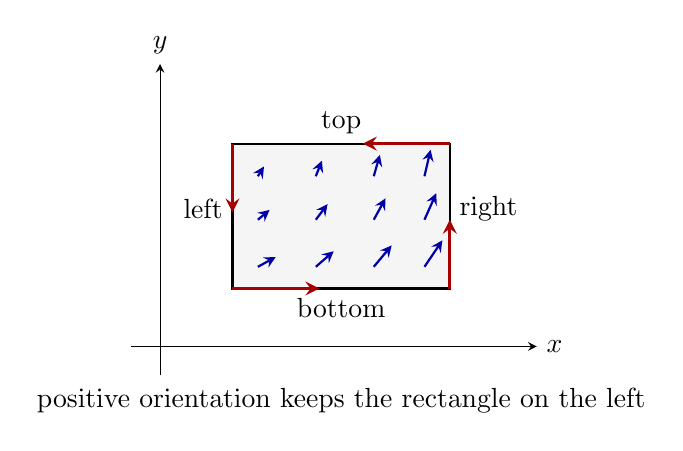
\begin{tikzpicture}[scale=0.92, >=stealth]
    \draw[->] (-0.4,0) -- (5.2,0) node[right] {\(x\)};
    \draw[->] (0,-0.4) -- (0,3.9) node[above] {\(y\)};

    \draw[thick, fill=gray!8] (1,0.8) rectangle (4,2.8);

    \draw[->, very thick, red!65!black] (1,0.8) -- (2.2,0.8);
    \draw[->, very thick, red!65!black] (4,0.8) -- (4,1.75);
    \draw[->, very thick, red!65!black] (4,2.8) -- (2.8,2.8);
    \draw[->, very thick, red!65!black] (1,2.8) -- (1,1.85);

    \node[below] at (2.5,0.8) {bottom};
    \node[right] at (4,1.9) {right};
    \node[above] at (2.5,2.8) {top};
    \node[left] at (1,1.9) {left};

    % Shifted the grid points slightly inwards and reduced the vector scale multipliers
    \foreach \x in {1.35,2.15,2.95,3.65} {
        \foreach \y in {1.1,1.75,2.35} {
            \draw[->, blue!65!black, thick]
                (\x,\y) -- ++({0.13*(3-\y)},{0.05*(2*\x)});
        }
    }

    \node at (2.5,-0.75) {positive orientation keeps the rectangle on the left};
\end{tikzpicture}
\caption{Circulation around a small rectangle compares opposite sides.}
\end{figure}

\subsection{The scalar curl in the plane}

The rectangle calculation generalizes.  On a small rectangle, the circulation of
\[
    \omega=P\,dx+Q\,dy
\]
is controlled by two rates:
\[
    Q_x,
    \qquad
    P_y.
\]

The right side and left side involve \(Q\,dy\).  If \(Q\) increases as \(x\) increases,
then the upward contribution on the right side is larger than the downward contribution
on the left side.  This contributes approximately
\[
    Q_x\,hk.
\]

The bottom and top involve \(P\,dx\).  The top is walked in the negative \(x\)-direction.
If \(P\) increases as \(y\) increases, then the top contribution cancels too much of the
bottom contribution.  This contributes approximately
\[
    -P_y\,hk.
\]

Together,
\[
\boxed{
    \oint_{\partial R}\omega
    \approx
    (Q_x-P_y)\,\Delta A
}
\]
for a small rectangle.

This coefficient gets its own name.

\begin{definition}[Scalar curl in the plane]
Let
\[
    \mathbf F(x,y)=(P(x,y),Q(x,y))
\]
be a vector field in the plane, and let
\[
    \omega=P\,dx+Q\,dy
\]
be its associated \(1\)-form.  The \emph{scalar curl} of \(\mathbf F\), or of \(\omega\), is
\[
\boxed{
    \operatorname{curl}_{\mathrm{plane}}\mathbf F
    =
    Q_x-P_y.
}
\]
\end{definition}

The word ``scalar'' matters.  In three-dimensional space, curl will be a vector.  In the
plane, the rotation axis points out of the page, so only one signed number is needed:
positive for counterclockwise tendency, negative for clockwise tendency.

For the form in the first example,
\[
    P=3-y,
    \qquad
    Q=2x.
\]
So
\[
    Q_x-P_y=2-(-1)=3,
\]
which matches the exact rectangle computation.

In the language of forms, the same coefficient appears in
\[
\boxed{
    d\omega=(Q_x-P_y)\,dx\wedge dy.
}
\]
Here \(dx\wedge dy\) measures signed area.  So \(d\omega\) is the signed circulation
per unit area.  This is why Chapter \ref{ch:13} kept pairing curl with the exterior
derivative.

\begin{example}[A shear field]
Let
\[
    \omega=x\,dy.
\]
Then
\[
    P=0,
    \qquad
    Q=x,
\]
so
\[
    Q_x-P_y=1.
\]
Around any small positively oriented rectangle, the circulation is approximately its
area.

For the rectangle
\[
    [a,a+h]\times[b,b+k],
\]
the computation is exact.  The bottom and top contribute nothing because \(dy=0\).
The right side contributes
\[
    (a+h)k,
\]
and the left side, walked downward, contributes
\[
    -ak.
\]
So
\[
\boxed{
    \oint_{\partial R}x\,dy=hk=\operatorname{Area}(R).
}
\]
This simple form will become an area-measuring tool in Green's theorem.
\end{example}

\subsection{Positive orientation of a plane region}

The sign of circulation depends on the direction of travel.  If we reverse a curve,
then
\[
    dx,
    \qquad dy
\]
reverse sign along the curve, and every \(1\)-form integral changes sign.

For a rectangle, the counterclockwise direction is the positive one.  For a general plane
region, the same idea is stated without mentioning clockwise or counterclockwise:

\begin{definition}[Positive orientation]
A boundary curve is \emph{positively oriented} if, as you walk along it, the region stays
on your left.
\end{definition}

For a region without holes, positive orientation usually means counterclockwise.
For a region with a hole, this rule has two effects:

\[
\begin{array}{c|c}
\text{boundary component} & \text{positive direction} \\ \hline
\text{outer boundary} & \text{counterclockwise}\\[1mm]
\text{inner boundary around a hole} & \text{clockwise}
\end{array}
\]

The clockwise direction on the inner boundary can feel surprising at first.  But if you
walk around a hole clockwise, the actual region, the material outside the hole, stays on
your left.

\begin{figure}[h]
\centering
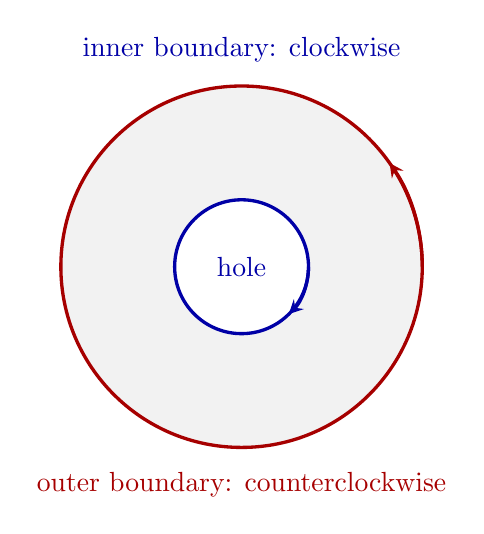
\begin{tikzpicture}[scale=0.85, >=stealth]
    \draw[fill=gray!10, even odd rule]
        (0,0) circle (2.7)
        (0,0) circle (1.0);

    \draw[very thick, red!65!black] (0,0) circle (2.7);
    \draw[->, very thick, red!65!black] (2.7,0) arc[start angle=0,end angle=35,radius=2.7];

    \draw[very thick, blue!65!black] (0,0) circle (1.0);
    \draw[->, very thick, blue!65!black] (1.0,0) arc[start angle=0,end angle=-45,radius=1.0];

    \node[red!65!black] at (0,-3.25) {outer boundary: counterclockwise};
    \node[blue!65!black] at (0,0) {hole};
    \node[blue!65!black] at (0,3.25) {inner boundary: clockwise};
\end{tikzpicture}
\caption{Positive orientation means the region stays on the left.  Inner boundaries are
oriented clockwise.}
\end{figure}

Orientation is not a convention we can ignore.  It is part of the theorem's sign.

\subsection{From many small rectangles to one boundary curve}

Now tile a region with many small rectangles.  Around each small rectangle,
\[
    \oint_{\partial R_i} \omega
    \approx
    (Q_x-P_y)\,\Delta A_i.
\]
Add these approximations over all rectangles:
\[
    \sum_i \oint_{\partial R_i}\omega
    \approx
    \sum_i (Q_x-P_y)\,\Delta A_i.
\]

The right side is becoming a double integral:
\[
    \sum_i (Q_x-P_y)\,\Delta A_i
    \longrightarrow
    \iint_R (Q_x-P_y)\,dA.
\]

The left side has a different kind of magic.  Every interior edge is walked twice: once
in one direction by one rectangle, and once in the opposite direction by the neighboring
rectangle.  Since line integrals reverse sign when orientation reverses, the two interior
edge contributions cancel.

Only the outside boundary survives.

\begin{figure}[h]
\centering
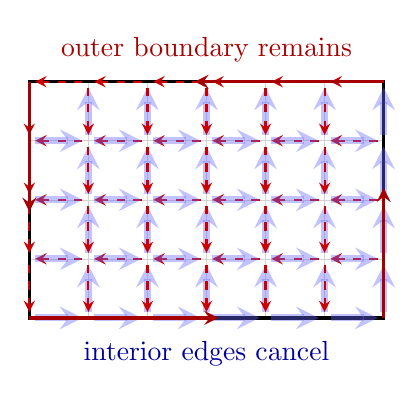
\begin{tikzpicture}[scale=0.75, >=stealth]
    % Light background grid and thick outer boundary
    \draw[step=1, gray!35, very thin] (0,0) grid (6,4);
    \draw[very thick] (0,0) rectangle (6,4);

    % Small circulation loops (colored by direction to show cancellation)
    \foreach \x in {0,...,5} {
        \foreach \y in {0,...,3} {
            % Forward/Positive directions (semitransparent thick blue)
            
            % Rightward (bottom edge)
            \draw[->, blue!60, line width=2.5pt, opacity=0.4]
                (\x+0.1, \y) -- (\x+0.9, \y);

            % Upward (right edge)
            \draw[->, blue!60, line width=2.5pt, opacity=0.4]
                (\x+1, \y+0.1) -- (\x+1, \y+0.9);

            % Reverse/Negative directions (dashed red)

            % Leftward (top edge)
            \draw[->, red!80!black, thick, dashed]
                (\x+0.9, \y+1) -- (\x+0.1, \y+1);

            % Downward (left edge)
            \draw[->, red!80!black, thick, dashed]
                (\x, \y+0.9) -- (\x, \y+0.1);
        }
    }

    % Macroscopic outer boundary arrows (drawn over the loops to unify the boundary)
    \draw[->, very thick, red!65!black] (0,0) -- (3.2,0);
    \draw[->, very thick, red!65!black] (6,0) -- (6,2.2);
    \draw[->, very thick, red!65!black] (6,4) -- (2.8,4);
    \draw[->, very thick, red!65!black] (0,4) -- (0,1.8);

    \node[blue!60!black] at (3,-0.6) {interior edges cancel};
    \node[red!65!black] at (3,4.55) {outer boundary remains};
\end{tikzpicture}
\caption{Adding circulation around small rectangles cancels all shared interior edges.}
\end{figure}

This cancellation is the beginning of Stokes' idea.  A sum of many tiny boundary
integrals becomes one large boundary integral.  A sum of many tiny curls becomes an
area integral.

The small-rectangle calculation has shown the mechanism.  The next step is to state
the theorem that says the limiting version is exact.

\section{Green's theorem: circulation form}
\label{sec:14.2}

Section \ref{sec:14.1} showed the engine: local circulation is measured by
\[
    Q_x-P_y,
\]
and shared interior edges cancel when rectangles are added.  Green's theorem says that
this engine works for a whole region, not only for a grid of rectangles.

Before the theorem, here is one complete example where both sides can be computed by
hand.

\subsection{A triangle that already contains the theorem}

Let \(T\) be the triangle with vertices
\[
    (0,0),\qquad (2,0),\qquad (0,1),
\]
listed counterclockwise.  Let
\[
    \omega=(x-y)\,dx+(x+2y)\,dy.
\]
Then
\[
    P=x-y,
    \qquad
    Q=x+2y,
\]
so
\[
    Q_x-P_y=1-(-1)=2.
\]
The area of the triangle is
\[
    \frac12(2)(1)=1.
\]
So the interior curl integral is
\[
\boxed{
    \iint_T (Q_x-P_y)\,dA
    =
    \iint_T 2\,dA
    =2.
}
\]

Now compute the boundary integral directly.

On the edge from \((0,0)\) to \((2,0)\), we have \(y=0\) and \(dy=0\), so
\[
    \int_0^2 x\,dx=2.
\]

On the edge from \((2,0)\) to \((0,1)\), use
\[
    x=2-2t,
    \qquad
    y=t,
    \qquad
    0\le t\le1.
\]
Then
\[
    dx=-2\,dt,
    \qquad
    dy=dt.
\]
Also
\[
    x-y=2-3t,
    \qquad
    x+2y=2.
\]
So
\[
\begin{aligned}
\int_{\text{slanted edge}}\omega
&=
\int_0^1\bigl[(2-3t)(-2)+2\bigr]dt\\
&=
\int_0^1(-2+6t)\,dt\\
&=1.
\end{aligned}
\]

On the edge from \((0,1)\) down to \((0,0)\), we have \(x=0\), \(dx=0\), and \(y\)
goes from \(1\) to \(0\).  Thus
\[
    \int_1^0 2y\,dy=-1.
\]

Adding the three edges gives
\[
\boxed{
    \oint_{\partial T}\omega
    =2+1-1=2.
}
\]
The boundary integral and the interior integral agree:
\[
\boxed{
    \oint_{\partial T}\omega
    =
    \iint_T (Q_x-P_y)\,dA.
}
\]

That is Green's theorem in one triangle.

\subsection{Statement of the theorem}

A region good enough for Green's theorem may have a curved boundary and may have
holes, but its boundary should be made from finitely many smooth pieces.  The field
should be differentiable on the region and slightly around it, so no singularity is hidden
on an edge or just inside the boundary.

\begin{theorem}[Green's theorem, circulation form]
Let \(R\) be a bounded plane region whose boundary \(\partial R\) consists of finitely
many piecewise smooth simple closed curves.  Give \(\partial R\) the positive
orientation, so the region stays on the left as the boundary is traversed.

Let
\[
    \omega=P\,dx+Q\,dy
\]
be a \(1\)-form whose coefficient functions \(P\) and \(Q\) have continuous first
partial derivatives on an open region containing \(R\).  Then
\[
\boxed{
    \oint_{\partial R} P\,dx+Q\,dy
    =
    \iint_R (Q_x-P_y)\,dA.
}
\]
Equivalently,
\[
\boxed{
    \oint_{\partial R}\omega
    =
    \iint_R d\omega,
    \qquad
    d\omega=(Q_x-P_y)\,dx\wedge dy.
}
\]
\end{theorem}

The first boxed formula is the classical vector-calculus version.  The second boxed
formula is the differential-forms version.  They say the same thing, but the forms
version shows the pattern that will later become Stokes' theorem.

The proof idea is the cancellation from Section \ref{sec:14.1}.  Prove the formula on
rectangles.  Cut a more complicated region into many small rectangles.  The interior
edge integrals cancel in pairs.  The small rectangle sums become the double integral of
\(Q_x-P_y\).  The remaining edge pieces approach the boundary integral around
\(\partial R\).  Section \ref{sec:14.5} will make this argument more careful.

\subsection{Why the hypotheses are doing work}

Each condition in the theorem protects the formula from a specific mistake.

\subsubsection*{Orientation cannot be reversed silently}

For the triangle example above,
\[
    \oint_{\partial T}\omega=2
\]
when \(\partial T\) is positively oriented.  If the same triangle is walked clockwise,
then the line integral becomes
\[
    -2.
\]
The interior integral is still
\[
    \iint_T 2\,dA=2.
\]
So Green's theorem would fail with the wrong sign.  The boundary orientation is part
of the statement, not a drawing choice.

\subsubsection*{A jump inside the region cannot be ignored}

Let
\[
    R=[-1,1]\times[0,1]
\]
and define
\[
    \omega=Q(x,y)\,dy,
    \qquad
    Q(x,y)=
    \begin{cases}
    0, & x\le0,\\
    1, & x>0.
    \end{cases}
\]
The form jumps along the vertical line \(x=0\).  It does not have continuous first
partial derivatives on \(R\).

Compute the boundary integral directly.  On the bottom and top edges, \(dy=0\).  On
the right edge, \(Q=1\) and \(y\) goes from \(0\) to \(1\), giving
\[
    \int_0^1 dy=1.
\]
On the left edge, \(Q=0\).  Therefore
\[
\boxed{
    \oint_{\partial R}\omega=1.
}
\]

Away from the jump line, \(Q_x=0\).  If we illegally pretended the curl were zero
everywhere, we would get
\[
    \iint_R 0\,dA=0,
\]
which is not the boundary integral.  The missing derivative along the jump line is
where the contribution lives.  The smoothness condition prevents this kind of hidden
edge inside the region.

\subsubsection*{A singularity inside the region changes the answer}

The form
\[
    \alpha=\frac{-y\,dx+x\,dy}{x^2+y^2}
\]
is defined on the punctured plane, but not at the origin.  On every point where it is
defined,
\[
    Q_x-P_y=0.
\]
Around the unit circle \(C\), oriented counterclockwise,
\[
    \oint_C \alpha=2\pi.
\]

If someone tried to apply Green's theorem to the disk bounded by \(C\), the right side
would seem to be
\[
    \iint_{\text{disk}}0\,dA=0,
\]
but the left side is \(2\pi\).  The theorem did not fail.  Its hypothesis failed: the form
is not defined on an open region containing the disk.  The origin is where the
circulation is hiding.

\subsection{Examples over simple regions}

Green's theorem is often useful because the boundary integral is hard while the area
integral is easy.

\begin{example}[A messy boundary integral around a disk]
Let \(D\) be the unit disk
\[
    x^2+y^2\le1,
\]
with positively oriented boundary.  Compute
\[
    \oint_{\partial D}(e^x-y^3)\,dx+(x^2+\sin y)\,dy.
\]

Here
\[
    P=e^x-y^3,
    \qquad
    Q=x^2+\sin y.
\]
So
\[
    Q_x=2x,
    \qquad
    P_y=-3y^2.
\]
Therefore
\[
    Q_x-P_y=2x+3y^2.
\]
Green's theorem gives
\[
\begin{aligned}
\oint_{\partial D}(e^x-y^3)\,dx+(x^2+\sin y)\,dy
&=
\iint_D(2x+3y^2)\,dA.
\end{aligned}
\]
By symmetry,
\[
    \iint_D 2x\,dA=0.
\]
Also,
\[
\begin{aligned}
\iint_D y^2\,dA
&=
\int_0^{2\pi}\int_0^1 r^2\sin^2\theta\,r\,dr\,d\theta\\
&=
\left(\int_0^1 r^3\,dr\right)
  \left(\int_0^{2\pi}\sin^2\theta\,d\theta\right)\\
&=
\frac14\cdot\pi\\
&=
\frac\pi4.
\end{aligned}
\]
Thus
\[
\boxed{
    \oint_{\partial D}(e^x-y^3)\,dx+(x^2+\sin y)\,dy
    =
    \frac{3\pi}{4}.
}
\]
The boundary integral would be unpleasant to compute directly.  The curl integral is
short.
\end{example}

\begin{example}[A rectangle where only the curl matters]
Let
\[
    R=[0,3]\times[0,2]
\]
and
\[
    \omega=(xy+\cos x)\,dx+(x^2+y^5)\,dy.
\]
Then
\[
    P_y=x,
    \qquad
    Q_x=2x.
\]
So
\[
    Q_x-P_y=x.
\]
Green's theorem gives
\[
\begin{aligned}
\oint_{\partial R}\omega
&=
\int_0^3\int_0^2 x\,dy\,dx\\
&=
\int_0^3 2x\,dx\\
&=9.
\end{aligned}
\]
The terms \(\cos x\) and \(y^5\) look large in the original form, but their contribution
to circulation around a closed boundary disappears because they do not affect
\(Q_x-P_y\).
\end{example}

\subsection{Using Green's theorem to compute area}

If we choose a \(1\)-form whose scalar curl is \(1\), then Green's theorem turns a
boundary integral into area.

Three common choices are
\[
    \omega=x\,dy,
\]
\[
    \omega=-y\,dx,
\]
and
\[
    \omega=\frac12(-y\,dx+x\,dy).
\]
Each has
\[
    Q_x-P_y=1.
\]
Therefore, for a positively oriented simple closed curve \(C=\partial R\),
\[
\boxed{
    \operatorname{Area}(R)
    =
    \oint_C x\,dy
    =
    -\oint_C y\,dx
    =
    \frac12\oint_C(-y\,dx+x\,dy).
}
\]

\begin{example}[The area of an ellipse from its boundary]
Let \(C\) be the ellipse
\[
    x=a\cos t,
    \qquad
    y=b\sin t,
    \qquad
    0\le t\le2\pi,
\]
where \(a>0\) and \(b>0\).  This parametrization is counterclockwise.

Use
\[
    \operatorname{Area}(R)=\oint_C x\,dy.
\]
Since
\[
    dy=b\cos t\,dt,
\]
we get
\[
\begin{aligned}
\operatorname{Area}(R)
&=
\int_0^{2\pi}(a\cos t)(b\cos t)\,dt\\
&=ab\int_0^{2\pi}\cos^2t\,dt\\
&=ab\pi.
\end{aligned}
\]
So
\[
\boxed{
    \operatorname{Area}(\text{ellipse})=\pi ab.
}
\]
A boundary integral has found the area inside the curve.
\end{example}

\subsection{Holes and multiple boundary components}

For a region with holes, \(\partial R\) means all boundary components with positive
orientation.  Leaving out an inner boundary changes the problem.

Let \(A\) be the annulus
\[
    1\le x^2+y^2\le4.
\]
Use again
\[
    \alpha=\frac{-y\,dx+x\,dy}{x^2+y^2}.
\]
This form is defined everywhere on the annulus, and
\[
    Q_x-P_y=0
\]
on the annulus.

The positively oriented boundary has two pieces:

\[
\begin{array}{c|c|c}
\text{boundary piece} & \text{radius} & \text{orientation} \\ \hline
C_{\mathrm{out}} & 2 & \text{counterclockwise}\\[1mm]
C_{\mathrm{in}} & 1 & \text{clockwise}
\end{array}
\]

Around any counterclockwise circle centered at the origin,
\[
    \int \alpha=2\pi.
\]
Therefore
\[
    \int_{C_{\mathrm{out}}}\alpha=2\pi,
\]
while the clockwise inner boundary gives
\[
    \int_{C_{\mathrm{in}}}\alpha=-2\pi.
\]
So
\[
\boxed{
    \oint_{\partial A}\alpha=2\pi-2\pi=0.
}
\]
This agrees with Green's theorem:
\[
\boxed{
    \iint_A 0\,dA=0.
}
\]

If we had used only the outer circle, we would have obtained \(2\pi\), but that would
not be the boundary of the annulus.  The inner boundary is not optional.  It is exactly
what records the hole.

Green's theorem has now turned circulation into an area integral.  But a vector field
near a closed curve can do another thing besides circulate around it.  It can cross the
curve outward or inward.  That second measurement is flux, and it leads to another
face of the same theorem: divergence in the plane.
\section{Green's theorem: flux form}
\label{sec:14.3}

Section \ref{sec:14.2} measured circulation.  A field could push us around a closed
curve, and Green's theorem turned that boundary circulation into the area integral of
the scalar curl:
\[
    \oint_{\partial R} P\,dx+Q\,dy
    =
    \iint_R (Q_x-P_y)\,dA.
\]

But a field near a boundary can do something else.  It can cross the boundary.  Fluid
can flow out of a pond.  Heat can leave a plate.  Air can escape through a closed
fence.  This measurement is called \emph{flux}.

\subsection{Outward normal in the plane}

Begin with a field that looks like a source:
\[
    \mathbf F(x,y)=(x,y).
\]
At every point, the arrow points away from the origin.  Let \(C\) be the circle of
radius \(a\), oriented counterclockwise:
\[
    \mathbf r(t)=(a\cos t,a\sin t),
    \qquad
    0\le t\le 2\pi.
\]
The outward unit normal on the circle is
\[
    \mathbf n(t)=(\cos t,\sin t).
\]
Along the circle,
\[
    \mathbf F(\mathbf r(t))=(a\cos t,a\sin t)=a\mathbf n(t).
\]
So the outward component of the field is
\[
    \mathbf F\cdot\mathbf n=a.
\]
Also,
\[
    ds=a\,dt.
\]
Therefore the total outward flux is
\[
\begin{aligned}
    \int_C \mathbf F\cdot\mathbf n\,ds
    &=
    \int_0^{2\pi} a(a\,dt)\\
    &=
    2\pi a^2.
\end{aligned}
\]
The disk inside the circle has area
\[
    \pi a^2.
\]
So in this example,
\[
\boxed{
    \int_C \mathbf F\cdot\mathbf n\,ds
    =
    2\,\operatorname{Area}(\text{disk}).
}
\]

The number \(2\) will soon get a name.  It is the divergence of
\[
    \mathbf F(x,y)=(x,y).
\]

\begin{figure}[h]
\centering
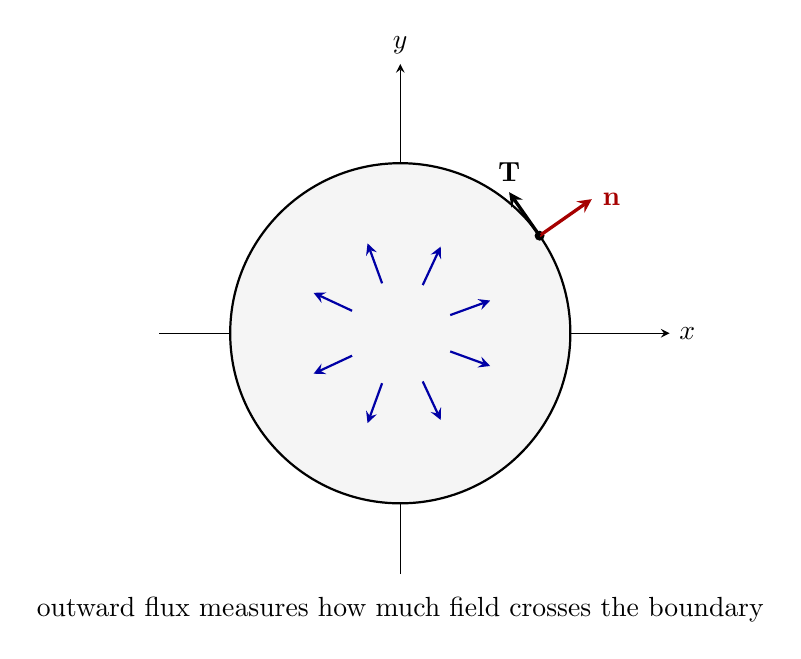
\begin{tikzpicture}[scale=0.9, >=stealth]
    \draw[->] (-3.4,0) -- (3.8,0) node[right] {\(x\)};
    \draw[->] (0,-3.4) -- (0,3.8) node[above] {\(y\)};

    \draw[thick, fill=gray!8] (0,0) circle (2.4);

    \foreach \ang in {20,65,110,155,205,250,295,340} {
        \draw[->, blue!65!black, thick]
            ({0.75*cos(\ang)},{0.75*sin(\ang)})
            -- ({1.35*cos(\ang)},{1.35*sin(\ang)});
    }

    \coordinate (P) at ({2.4*cos(35)},{2.4*sin(35)});
    \fill (P) circle (2pt);

    \draw[->, very thick, red!65!black]
        (P) -- ++({0.9*cos(35)},{0.9*sin(35)})
        node[right] {\(\mathbf n\)};

    \draw[->, very thick]
        (P) -- ++({-0.75*sin(35)},{0.75*cos(35)})
        node[above] {\(\mathbf T\)};

    \node at (0,-3.9) {outward flux measures how much field crosses the boundary};
\end{tikzpicture}
\caption{For the radial field \(\mathbf F=(x,y)\), the arrows point outward through the
circle.}
\end{figure}

For a general positively oriented boundary curve, the outward normal has a simple
formula.

Suppose
\[
    C=\partial R
\]
is positively oriented, so the region stays on the left as we walk.  Let
\[
    \mathbf T=\left(\frac{dx}{ds},\frac{dy}{ds}\right)
\]
be the unit tangent vector.  Since the region is on the left, the left normal points
inward.  The outward normal is the right normal:
\[
\boxed{
    \mathbf n=
    \left(
        \frac{dy}{ds},
        -\frac{dx}{ds}
    \right).
}
\]
Therefore, if
\[
    \mathbf F=(M,N),
\]
then
\[
\begin{aligned}
    \mathbf F\cdot\mathbf n\,ds
    &=
    (M,N)\cdot
    \left(
        \frac{dy}{ds},
        -\frac{dx}{ds}
    \right)ds\\
    &=
    M\,dy-N\,dx.
\end{aligned}
\]
So for a positively oriented boundary,
\[
\boxed{
    \int_{\partial R}\mathbf F\cdot\mathbf n\,ds
    =
    \oint_{\partial R} M\,dy-N\,dx.
}
\]

This formula is useful because it removes the square root hidden in \(ds\).  It also
reveals that flux is another \(1\)-form integral.

\begin{definition}[Flux across a plane curve]
Let \(C\) be an oriented curve with a chosen unit normal \(\mathbf n\), and let
\[
    \mathbf F=(M,N)
\]
be a vector field.  The \emph{flux} of \(\mathbf F\) across \(C\) is
\[
\boxed{
    \int_C \mathbf F\cdot\mathbf n\,ds.
}
\]
If \(C=\partial R\), the normal is usually chosen to be the outward normal.
\end{definition}

For a closed curve, outward flux is positive when more field leaves the region than
enters it.  It is negative when more field enters than leaves.

\subsection{Divergence in two dimensions}

Now look at a small rectangle
\[
    S=[a,a+h]\times[b,b+k].
\]
Let
\[
    \mathbf F=(M,N).
\]
The horizontal component \(M\) contributes to flux through the vertical sides.  The
vertical component \(N\) contributes to flux through the horizontal sides.

On the right side, the outward normal points right, so the contribution is roughly
\[
    M(a+h,b)\,k.
\]
On the left side, the outward normal points left, so the contribution is roughly
\[
    -M(a,b)\,k.
\]
Together the vertical sides contribute approximately
\[
    \bigl(M(a+h,b)-M(a,b)\bigr)k
    \approx
    M_x(a,b)\,h\,k.
\]

On the top side, the outward normal points up, so the contribution is roughly
\[
    N(a,b+k)\,h.
\]
On the bottom side, the outward normal points down, so the contribution is roughly
\[
    -N(a,b)\,h.
\]
Together the horizontal sides contribute approximately
\[
    \bigl(N(a,b+k)-N(a,b)\bigr)h
    \approx
    N_y(a,b)\,k\,h.
\]

Adding all four sides,
\[
\boxed{
    \int_{\partial S}\mathbf F\cdot\mathbf n\,ds
    \approx
    (M_x+N_y)\,\Delta A.
}
\]

This coefficient is the local net outflow per unit area.

\begin{definition}[Divergence in the plane]
Let
\[
    \mathbf F(x,y)=(M(x,y),N(x,y))
\]
be a vector field in the plane.  The \emph{divergence} of \(\mathbf F\) is
\[
\boxed{
    \operatorname{div}\mathbf F
    =
    \nabla\cdot\mathbf F
    =
    M_x+N_y.
}
\]
\end{definition}

For the radial source
\[
    \mathbf F(x,y)=(x,y),
\]
we get
\[
    \operatorname{div}\mathbf F=1+1=2,
\]
which matches the circle computation:
\[
    \text{outward flux}=2\cdot\text{area}.
\]

The divergence measures source strength.  Positive divergence means local net outflow.
Negative divergence means local net inflow.  Zero divergence means that, to first
order, what flows into a tiny region also flows out.

\begin{example}[A field with circulation but no divergence]
Let
\[
    \mathbf F(x,y)=(-y,x).
\]
Then
\[
    \operatorname{div}\mathbf F
    =
    \frac{\partial}{\partial x}(-y)
    +
    \frac{\partial}{\partial y}(x)
    =
    0.
\]
This field circulates around the origin, but it has no local source or sink.

In Section \ref{sec:14.1}, the same field had scalar curl
\[
    Q_x-P_y=1-(-1)=2.
\]
So curl and divergence measure different behavior:
\[
\begin{array}{c|c}
\text{curl} & \text{tendency to circulate}\\[1mm]
\text{divergence} & \text{tendency to flow outward}
\end{array}
\]
\end{example}

\subsection{Green's theorem in flux form}

The small-rectangle calculation suggests the theorem.  The flux through the boundary
should equal the integral of divergence over the inside.

\begin{theorem}[Green's theorem, flux form]
Let \(R\) be a bounded plane region whose boundary \(\partial R\) consists of finitely
many piecewise smooth simple closed curves.  Give \(\partial R\) the positive
orientation, and let \(\mathbf n\) be the outward unit normal.

Let
\[
    \mathbf F=(M,N)
\]
be a vector field whose component functions have continuous first partial derivatives
on an open region containing \(R\).  Then
\[
\boxed{
    \oint_{\partial R}\mathbf F\cdot\mathbf n\,ds
    =
    \iint_R (M_x+N_y)\,dA.
}
\]
Equivalently,
\[
\boxed{
    \oint_{\partial R} M\,dy-N\,dx
    =
    \iint_R (M_x+N_y)\,dA.
}
\]
\end{theorem}

This is not a separate miracle from the circulation form of Green's theorem.  It is the
same theorem applied to the \(1\)-form
\[
    \omega=-N\,dx+M\,dy.
\]
For this form,
\[
    P=-N,
    \qquad
    Q=M.
\]
So
\[
    Q_x-P_y
    =
    M_x-(-N_y)
    =
    M_x+N_y.
\]
The circulation form says
\[
    \oint_{\partial R} -N\,dx+M\,dy
    =
    \iint_R (M_x+N_y)\,dA,
\]
which is exactly the flux form.

\subsection{Examples of net outflow}

\begin{example}[A steady wind through a closed fence]
Let
\[
    \mathbf F(x,y)=(5,2)
\]
be a constant wind field.  Then
\[
    \operatorname{div}\mathbf F=0+0=0.
\]
For any region \(R\) to which Green's theorem applies,
\[
\boxed{
    \oint_{\partial R}\mathbf F\cdot\mathbf n\,ds=0.
}
\]
This does not mean no wind crosses the fence.  Wind enters one side and leaves another.
The theorem says the total entering and total leaving cancel.
\end{example}

\begin{example}[Flux through an ellipse without parametrizing the ellipse]
Let \(E\) be the elliptical region
\[
    \frac{x^2}{a^2}+\frac{y^2}{b^2}\le 1,
\]
where \(a,b>0\).  Let
\[
    \mathbf F(x,y)=(x+\sin y,\;y+e^x).
\]
A direct flux integral around the ellipse would be unpleasant.  Green's theorem makes
it short.

Here
\[
    M=x+\sin y,
    \qquad
    N=y+e^x.
\]
Therefore
\[
    M_x=1,
    \qquad
    N_y=1.
\]
So
\[
    \operatorname{div}\mathbf F=2.
\]
Hence
\[
\begin{aligned}
    \oint_{\partial E}\mathbf F\cdot\mathbf n\,ds
    &=
    \iint_E 2\,dA\\
    &=
    2\,\operatorname{Area}(E)\\
    &=
    2\pi ab.
\end{aligned}
\]
Thus
\[
\boxed{
    \oint_{\partial E}\mathbf F\cdot\mathbf n\,ds=2\pi ab.
}
\]
The extra terms \(\sin y\) and \(e^x\) affect the boundary arrows, but they do not
change the divergence in this example.
\end{example}

\begin{example}[A sink]
Let
\[
    R=[0,2]\times[0,1]
\]
and
\[
    \mathbf F(x,y)=(-2x,-3y).
\]
Then
\[
    \operatorname{div}\mathbf F=-2-3=-5.
\]
Green's theorem gives
\[
\begin{aligned}
    \oint_{\partial R}\mathbf F\cdot\mathbf n\,ds
    &=
    \iint_R (-5)\,dA\\
    &=
    -5\cdot 2\\
    &=
    -10.
\end{aligned}
\]
So
\[
\boxed{
    \oint_{\partial R}\mathbf F\cdot\mathbf n\,ds=-10.
}
\]
The negative sign says that, in total, more field enters the rectangle than leaves it.
\end{example}

\subsection{Why the hypotheses are doing work}

The flux form has the same kind of hypotheses as the circulation form.  They keep
hidden sources and hidden boundaries from being smuggled into the region.

\subsubsection*{The outward normal cannot be replaced by the inward normal}

For
\[
    \mathbf F=(x,y)
\]
on the disk of radius \(a\),
\[
    \oint_{\partial R}\mathbf F\cdot\mathbf n\,ds=2\pi a^2
\]
with the outward normal.  If we use the inward normal instead, the answer becomes
\[
    -2\pi a^2.
\]
The interior integral
\[
    \iint_R 2\,dA
\]
does not change.  The theorem is about outward flux.

\subsubsection*{A jump inside the region can hide a source line}

Let
\[
    R=[-1,1]\times[0,1]
\]
and define
\[
    \mathbf F(x,y)=
    \begin{cases}
    (0,0), & x\le0,\\
    (1,0), & x>0.
    \end{cases}
\]
This field jumps across the line \(x=0\).  It is not \(C^1\).

The boundary flux is easy.  The right side has outward normal \((1,0)\), so it
contributes
\[
    1.
\]
The left side has field \((0,0)\), and the top and bottom have normals perpendicular
to the field.  Therefore
\[
\boxed{
    \oint_{\partial R}\mathbf F\cdot\mathbf n\,ds=1.
}
\]

Away from the jump line,
\[
    M_x+N_y=0.
\]
If we illegally ignored the jump and integrated \(0\), we would get
\[
    \iint_R 0\,dA=0.
\]
The missing contribution lives on the internal jump line.  The smoothness hypothesis
prevents an unseen boundary from appearing inside the region.

\subsubsection*{A singularity can hide a point source}

Consider the radial field
\[
    \mathbf F(x,y)=\frac{1}{x^2+y^2}(x,y).
\]
It is defined on the punctured plane, but not at the origin.  Away from the origin,
\[
    \operatorname{div}\mathbf F=0.
\]
On the unit circle,
\[
    \mathbf F=(\cos t,\sin t)=\mathbf n,
\]
and
\[
    ds=dt.
\]
So
\[
\boxed{
    \oint_C \mathbf F\cdot\mathbf n\,ds=2\pi.
}
\]
If we tried to apply Green's theorem to the whole unit disk, the right side would seem
to be \(0\), while the boundary flux is \(2\pi\).  The theorem did not fail.  The field is
not defined on an open region containing the disk.  The origin is a hidden source.

If we instead use the annulus
\[
    \varepsilon\le x^2+y^2\le1,
\]
then the field is defined on the region.  The outer boundary contributes \(2\pi\), and
the inner boundary, whose outward normal points into the hole, contributes
\[
    -2\pi.
\]
The total flux is \(0\), exactly matching
\[
    \iint_{\text{annulus}}0\,dA=0.
\]
The inner boundary is what records the missing point.

\subsection{Source, sink, and net outflow interpretations}

For a small region around a point,
\[
    \operatorname{div}\mathbf F
\]
is the net outward flux per unit area.

If
\[
    \operatorname{div}\mathbf F>0,
\]
the point behaves like a source.  More field leaves a tiny box than enters it.

If
\[
    \operatorname{div}\mathbf F<0,
\]
the point behaves like a sink.  More field enters than leaves.

If
\[
    \operatorname{div}\mathbf F=0,
\]
there is no first-order net creation or loss.  The field may still move, shear, stretch,
or rotate, but it is not locally adding or removing material.

Green's theorem now has two faces:
\[
\begin{array}{c|c|c}
\text{Boundary measurement} & \text{Interior density} & \text{Name}\\ \hline
\displaystyle \oint_{\partial R} P\,dx+Q\,dy
&
\displaystyle Q_x-P_y
&
\text{circulation / curl}\\[3mm]
\displaystyle \oint_{\partial R} M\,dy-N\,dx
&
\displaystyle M_x+N_y
&
\text{flux / divergence}
\end{array}
\]

The two formulas look different, but the boundary integrals are both \(1\)-form
integrals.  The real unifying object is not the vector field.  It is the form being
integrated around the boundary.  Once we focus on that form, Green's theorem becomes
one sentence.

\section{Green's theorem in differential-form language}
\label{sec:14.4}

The circulation form and the flux form of Green's theorem are two costumes for the
same idea.  In both cases, a \(1\)-form is integrated around a boundary, and its exterior
derivative is integrated over the region inside.

The notation is shorter:
\[
    \int_{\partial R}\omega=\int_R d\omega.
\]
But the meaning is the same story we have been building: boundary accumulation equals
interior accumulation of a derivative.

\subsection{A \(1\)-form on the boundary}

Recall from Section \ref{sec:13.4} that a \(1\)-form in the plane has the form
\[
    \omega=P\,dx+Q\,dy.
\]
It is built to be integrated along a curve.  At each tiny step, it reads the \(x\)-change
and \(y\)-change, weights them by \(P\) and \(Q\), and adds.

For a vector field
\[
    \mathbf F=(M,N),
\]
there are two natural \(1\)-forms one might build.

The work or circulation form is
\[
\boxed{
    \omega_{\mathrm{work}}=M\,dx+N\,dy.
}
\]
It measures motion along the curve:
\[
    \int_C \omega_{\mathrm{work}}
    =
    \int_C \mathbf F\cdot d\mathbf r.
\]

The flux form is
\[
\boxed{
    \omega_{\mathrm{flux}}=M\,dy-N\,dx.
}
\]
When \(C=\partial R\) is positively oriented, it measures outward crossing:
\[
    \int_{\partial R}\omega_{\mathrm{flux}}
    =
    \oint_{\partial R}\mathbf F\cdot\mathbf n\,ds.
\]

So the same vector field can give two different boundary measurements.  The difference
is not in the field alone.  It is in the \(1\)-form we choose to integrate.

\[
\begin{array}{c|c|c}
\text{Measurement} & \text{\(1\)-form} & \text{What it reads}\\ \hline
\text{work/circulation} & M\,dx+N\,dy & \text{motion along the curve}\\[1mm]
\text{flux} & M\,dy-N\,dx & \text{motion through the curve}
\end{array}
\]

This is why forms are useful.  They remember the actual integrand.

\subsection{The exterior derivative in the plane}

Take the form
\[
    \omega=(x-y)\,dx+(x+2y)\,dy.
\]
This is the form from the triangle example in Section \ref{sec:14.2}.  There,
\[
    P=x-y,
    \qquad
    Q=x+2y.
\]
The coefficient that appeared in Green's theorem was
\[
    Q_x-P_y=1-(-1)=2.
\]
So the interior form was
\[
    2\,dx\wedge dy.
\]
That is the exterior derivative of \(\omega\):
\[
\boxed{
    d\omega=2\,dx\wedge dy.
}
\]

Now write the general rule.

\begin{definition}[Exterior derivative of a plane \(1\)-form]
Let
\[
    \omega=P(x,y)\,dx+Q(x,y)\,dy
\]
be a \(C^1\) \(1\)-form in the plane.  Its \emph{exterior derivative} is the \(2\)-form
\[
\boxed{
    d\omega=(Q_x-P_y)\,dx\wedge dy.
}
\]
\end{definition}

The coefficient
\[
    Q_x-P_y
\]
is the scalar curl of the form
\[
    P\,dx+Q\,dy.
\]
The factor
\[
    dx\wedge dy
\]
is the signed area form.

Here is the same rule expanded once, so the signs are not mysterious.  Since
\[
    dP=P_x\,dx+P_y\,dy,
\]
and
\[
    dQ=Q_x\,dx+Q_y\,dy,
\]
we compute
\[
\begin{aligned}
    d(P\,dx+Q\,dy)
    &=
    dP\wedge dx+dQ\wedge dy\\
    &=
    (P_x\,dx+P_y\,dy)\wedge dx
    +
    (Q_x\,dx+Q_y\,dy)\wedge dy\\
    &=
    P_y\,dy\wedge dx+Q_x\,dx\wedge dy\\
    &=
    -P_y\,dx\wedge dy+Q_x\,dx\wedge dy\\
    &=
    (Q_x-P_y)\,dx\wedge dy.
\end{aligned}
\]
The terms involving
\[
    dx\wedge dx
    \qquad\text{and}\qquad
    dy\wedge dy
\]
vanish because a parallelogram with two identical directions has zero signed area.

\begin{example}[The area-measuring form]
Let
\[
    \eta=-y\,dx+x\,dy.
\]
Then
\[
    P=-y,
    \qquad
    Q=x.
\]
So
\[
    d\eta=(1-(-1))\,dx\wedge dy=2\,dx\wedge dy.
\]
Green's theorem says
\[
    \oint_{\partial R}\eta
    =
    \iint_R 2\,dx\wedge dy.
\]
Thus
\[
    \oint_{\partial R}(-y\,dx+x\,dy)
    =
    2\,\operatorname{Area}(R)
\]
for a positively oriented simple boundary.  This is exactly the pattern Chapter
\ref{ch:13} discovered before Green's theorem gave it a name.
\end{example}

\subsection{Green's theorem as one formula}

Now the circulation form of Green's theorem becomes a single statement.

\begin{theorem}[Green's theorem for \(1\)-forms]
Let \(R\) be a bounded plane region whose boundary consists of finitely many
piecewise smooth simple closed curves, with positive orientation.

Let
\[
    \omega=P\,dx+Q\,dy
\]
be a \(C^1\) \(1\)-form on an open region containing \(R\).  Then
\[
\boxed{
    \int_{\partial R}\omega
    =
    \int_R d\omega.
}
\]
Written out in coordinates, this says
\[
\boxed{
    \oint_{\partial R} P\,dx+Q\,dy
    =
    \iint_R (Q_x-P_y)\,dx\wedge dy.
}
\]
\end{theorem}

The symbol
\[
    \int_R d\omega
\]
means an integral of the \(2\)-form
\[
    d\omega
\]
over the oriented region \(R\).  For the standard counterclockwise orientation of the
plane,
\[
    dx\wedge dy
\]
agrees with positive area, so this is the same number as
\[
    \iint_R (Q_x-P_y)\,dA.
\]

\begin{figure}[h]
\centering
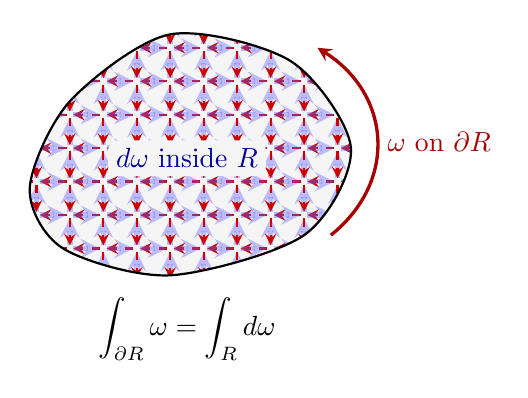
\begin{tikzpicture}[scale=0.85, >=stealth]
    
    % 1. Clipping region for the internal circulation grid
    \begin{scope}
        \clip plot[smooth cycle] coordinates {
            (0.4,0.5) (2.0,0.1) (4.0,0.7) (4.7,2.0)
            (3.8,3.3) (2.0,3.7) (0.5,2.7) (-0.1,1.4)
        };
        
        \fill[gray!8] (-1,-1) rectangle (6,5);

        % Dense grid of circulation cells 
        \foreach \x in {-0.5, 0.0, 0.5, 1.0, 1.5, 2.0, 2.5, 3.0, 3.5, 4.0, 4.5} {
            \foreach \y in {-0.5, 0.0, 0.5, 1.0, 1.5, 2.0, 2.5, 3.0, 3.5} {
                % Forward/Positive directions 
                \draw[->, blue!60, line width=2pt, opacity=0.4] 
                    (\x+0.05, \y) -- (\x+0.45, \y);
                \draw[->, blue!60, line width=2pt, opacity=0.4] 
                    (\x+0.5, \y+0.05) -- (\x+0.5, \y+0.45);
                    
                % Reverse/Negative directions 
                \draw[->, red!80!black, thick, dashed] 
                    (\x+0.45, \y+0.5) -- (\x+0.05, \y+0.5);
                \draw[->, red!80!black, thick, dashed] 
                    (\x, \y+0.45) -- (\x, \y+0.05);
            }
        }
    \end{scope}

    % 2. Draw the macroscopic outer boundary cleanly
    \draw[thick]
        plot[smooth cycle] coordinates {
            (0.4,0.5) (2.0,0.1) (4.0,0.7) (4.7,2.0)
            (3.8,3.3) (2.0,3.7) (0.5,2.7) (-0.1,1.4)
        };

    % 3. Single long red arrow to indicate orientation (hovering cleanly outside the boundary)
    \draw[->, very thick, red!65!black] 
        (4.4, 0.7) .. controls (5.4, 1.5) and (5.3, 2.8) .. (4.2, 3.5);

    % 4. Labels
    \node[red!65!black, right] at (5.1, 2.1) {\(\omega\) on \(\partial R\)};
    
    \node[blue!60!black, fill=gray!8, inner sep=3pt, rounded corners] at (2.25,1.85) {\(d\omega\) inside \(R\)};

    \node at (2.25,-0.7) {\(\displaystyle \int_{\partial R}\omega=\int_R d\omega\)};
\end{tikzpicture}
\caption{Green's theorem says that a boundary integral of a \(1\)-form equals an
interior integral of its exterior derivative.}
\end{figure}

The two versions of Green's theorem now sit in one table.

\[
\begin{array}{c|c|c}
\text{Boundary form} & \text{Exterior derivative} & \text{Interior meaning}\\ \hline
M\,dx+N\,dy
&
(N_x-M_y)\,dx\wedge dy
&
\text{curl density}\\[1mm]
M\,dy-N\,dx
&
(M_x+N_y)\,dx\wedge dy
&
\text{divergence density}
\end{array}
\]

The same vector field \((M,N)\) can be used in either row.  The form decides what
kind of boundary measurement we are making.

\begin{example}[Flux as a form calculation]
Let
\[
    \mathbf F=(M,N)=(x+\sin y,\;y+e^x).
\]
The flux form is
\[
    \omega_{\mathrm{flux}}=M\,dy-N\,dx
    =
    (x+\sin y)\,dy-(y+e^x)\,dx.
\]
Written as
\[
    P\,dx+Q\,dy,
\]
this has
\[
    P=-(y+e^x),
    \qquad
    Q=x+\sin y.
\]
Therefore
\[
\begin{aligned}
d\omega_{\mathrm{flux}}
&=
(Q_x-P_y)\,dx\wedge dy\\
&=
(1-(-1))\,dx\wedge dy\\
&=
2\,dx\wedge dy.
\end{aligned}
\]
So for any positively oriented region \(R\),
\[
    \oint_{\partial R}\omega_{\mathrm{flux}}
    =
    \iint_R 2\,dx\wedge dy
    =
    2\,\operatorname{Area}(R).
\]
This is the flux theorem again, because
\[
    M_x+N_y=1+1=2.
\]
\end{example}

\subsection{The warnings are part of the formula}

The compact formula
\[
    \int_{\partial R}\omega=\int_R d\omega
\]
is easy to remember.  It is also easy to misuse.

The form must be defined and smooth on a region containing \(R\).  The boundary must
carry the correct orientation.  All boundary components must be included.

The punctured-plane form
\[
    \alpha=\frac{-y\,dx+x\,dy}{x^2+y^2}
\]
is the cleanest warning.  On the punctured plane,
\[
    d\alpha=0.
\]
But on the unit circle,
\[
    \oint_C \alpha=2\pi.
\]
We cannot apply Green's theorem to the whole disk because \(\alpha\) is not defined at
the origin.

If the region is an annulus around the origin, then the theorem works.  The positively
oriented boundary has two pieces: the outer circle counterclockwise and the inner
circle clockwise.  The two integrals are
\[
    2\pi
    \qquad\text{and}\qquad
    -2\pi,
\]
so the total is
\[
    0.
\]
That agrees with
\[
    \int_R d\alpha=\int_R 0=0.
\]
The short formula is trustworthy only when its hypotheses are present.

\subsection{Why this is already Stokes' theorem in disguise}

The Fundamental Theorem of Calculus can be written in the same shape.

On an interval \([a,b]\), a function \(f\) has differential
\[
    df=f'(x)\,dx.
\]
The boundary of the interval is the endpoint \(b\) with positive sign and the endpoint
\(a\) with negative sign.  So
\[
    \int_{\partial [a,b]} f=f(b)-f(a).
\]
The Fundamental Theorem of Calculus says
\[
\boxed{
    \int_{\partial [a,b]} f
    =
    \int_{[a,b]} df.
}
\]
Written out,
\[
    f(b)-f(a)
    =
    \int_a^b f'(x)\,dx.
\]

Green's theorem says the same kind of thing one dimension higher:
\[
\boxed{
    \int_{\partial R}\omega
    =
    \int_R d\omega.
}
\]

\[
\begin{array}{c|c|c|c}
\text{Dimension} & \text{Region} & \text{Boundary object} & \text{Interior derivative}\\ \hline
1 & [a,b] & f & df\\[1mm]
2 & R & \omega & d\omega
\end{array}
\]

This is the beginning of Stokes' idea.  The boundary of a region carries one kind of
integrand.  The inside carries its exterior derivative.  The integral over the boundary
equals the integral over the inside.

Later, a surface in space will have a boundary curve, and a solid in space will have a
boundary surface.  The same sentence will survive both times.  What changes is the
kind of form being integrated.

The formula is beautiful enough to make us suspicious: why should all the interior
information collapse to the boundary?  The answer is not magic.  Cut the region into
many small rectangles.  Every shared interior edge is walked twice, in opposite
directions, and disappears.  The proof of Green's theorem is the art of making that
cancellation honest.
\section{Why Green's theorem is true}
\label{sec:14.5}

Section \ref{sec:14.4} compressed Green's theorem into one line:
\[
    \int_{\partial R}\omega=\int_R d\omega.
\]
The formula is short, but it is not magic.  It comes from two old facts working
together:

\[
\begin{array}{c|c}
\text{old fact} & \text{new role}\\ \hline
\text{the Fundamental Theorem of Calculus} & \text{turns edge differences into derivatives}\\[1mm]
\text{opposite orientations cancel} & \text{removes all interior edges}
\end{array}
\]

Both facts can already be seen on one rectangle.

\subsection{A rectangle with only vertical motion}

Start with the form
\[
    \omega=(x^2+y)\,dy
\]
on the rectangle
\[
    R=[0,2]\times[0,1].
\]
Only the vertical sides matter, because \(dy=0\) along horizontal sides.

On the right side,
\[
    x=2,
    \qquad
    0\le y\le1,
\]
so
\[
\begin{aligned}
    \int_{\text{right}}\omega
    &=
    \int_0^1(4+y)\,dy\\
    &=
    4+\frac12.
\end{aligned}
\]
On the left side, positive orientation walks downward:
\[
    x=0,
    \qquad
    1\ge y\ge0.
\]
Thus
\[
\begin{aligned}
    \int_{\text{left}}\omega
    &=
    \int_1^0 y\,dy\\
    &=
    -\frac12.
\end{aligned}
\]
Therefore
\[
\boxed{
    \oint_{\partial R}(x^2+y)\,dy=4.
}
\]

Now compute the interior side.  Since
\[
    P=0,
    \qquad
    Q=x^2+y,
\]
we have
\[
    d\omega=Q_x\,dx\wedge dy=2x\,dx\wedge dy.
\]
So
\[
\begin{aligned}
    \iint_R d\omega
    &=
    \int_0^2\int_0^1 2x\,dy\,dx\\
    &=
    \int_0^2 2x\,dx\\
    &=
    4.
\end{aligned}
\]
The two answers agree:
\[
\boxed{
    \oint_{\partial R}\omega=\iint_R d\omega.
}
\]

What happened?  The boundary integral compared the value of \(Q\) on the right side
with the value of \(Q\) on the left side:
\[
    Q(2,y)-Q(0,y).
\]
The Fundamental Theorem of Calculus rewrites that difference as
\[
    Q(2,y)-Q(0,y)=\int_0^2 Q_x(x,y)\,dx.
\]
Then integrating over \(y\) gives the double integral.

\subsection{The proof for a rectangle}

Now let
\[
    R=[a,b]\times[c,d],
\]
and let
\[
    \omega=P\,dx+Q\,dy
\]
where \(P\) and \(Q\) have continuous first partial derivatives.

First look at the \(Q\,dy\) part.  Along the bottom and top edges, \(dy=0\).  The right
side contributes
\[
    \int_c^d Q(b,y)\,dy,
\]
and the left side, walked downward, contributes
\[
    \int_d^c Q(a,y)\,dy
    =
    -\int_c^d Q(a,y)\,dy.
\]
So
\[
\begin{aligned}
    \oint_{\partial R} Q\,dy
    &=
    \int_c^d \bigl(Q(b,y)-Q(a,y)\bigr)\,dy.
\end{aligned}
\]
For each fixed \(y\), the single-variable Fundamental Theorem of Calculus gives
\[
    Q(b,y)-Q(a,y)=\int_a^b Q_x(x,y)\,dx.
\]
Therefore
\[
\boxed{
    \oint_{\partial R}Q\,dy
    =
    \int_c^d\int_a^b Q_x(x,y)\,dx\,dy.
}
\]

Now look at the \(P\,dx\) part.  Along the vertical sides, \(dx=0\).  The bottom side is
walked from \(a\) to \(b\), and the top side is walked from \(b\) to \(a\).  Hence
\[
\begin{aligned}
    \oint_{\partial R} P\,dx
    &=
    \int_a^b P(x,c)\,dx+\int_b^a P(x,d)\,dx\\
    &=
    \int_a^b \bigl(P(x,c)-P(x,d)\bigr)\,dx.
\end{aligned}
\]
For each fixed \(x\),
\[
    P(x,d)-P(x,c)=\int_c^d P_y(x,y)\,dy.
\]
Thus
\[
    P(x,c)-P(x,d)
    =
    -\int_c^d P_y(x,y)\,dy.
\]
So
\[
\boxed{
    \oint_{\partial R}P\,dx
    =
    -\int_a^b\int_c^d P_y(x,y)\,dy\,dx.
}
\]

Adding the two parts gives
\[
\boxed{
    \oint_{\partial R}P\,dx+Q\,dy
    =
    \iint_R (Q_x-P_y)\,dA.
}
\]
In form language,
\[
\boxed{
    \int_{\partial R}\omega=\int_R d\omega.
}
\]

The rectangle proof is just the Fundamental Theorem of Calculus applied once in the
\(x\)-direction and once in the \(y\)-direction.  The signs come from orientation.

\subsection{Two rectangles and one disappearing edge}

A single rectangle explains where \(Q_x-P_y\) comes from.  The next idea explains why
only the outside boundary survives.

Put two rectangles side by side:
\[
    R_1=[0,1]\times[0,1],
    \qquad
    R_2=[1,2]\times[0,1].
\]
They share the vertical edge
\[
    E=\{1\}\times[0,1].
\]
For \(R_1\), positive orientation walks up along \(E\).  For \(R_2\), positive orientation
walks down along the same edge.

Along \(E\),
\[
    x=1,
    \qquad
    dx=0.
\]
So the contribution from \(R_1\) is
\[
    \int_0^1 Q(1,y)\,dy.
\]
The contribution from \(R_2\) is
\[
    \int_1^0 Q(1,y)\,dy.
\]
They add to zero.

\[
\boxed{
    \int_E Q\,dy+\int_{-E}Q\,dy=0.
}
\]

The same cancellation happens for any shared edge.  One rectangle walks the edge in
one direction; the neighboring rectangle walks it in the opposite direction.  A line
integral changes sign when orientation reverses, so the two contributions cancel.

\begin{figure}[h]
\centering
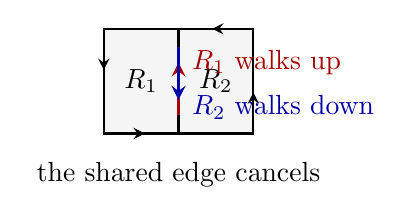
\begin{tikzpicture}[scale=0.95, >=stealth]
    \draw[fill=gray!8] (0,0) rectangle (2,1.4);
    \draw[thick] (0,0) rectangle (2,1.4);
    \draw[thick] (1,0) -- (1,1.4);

    \node at (0.5,0.7) {\(R_1\)};
    \node at (1.5,0.7) {\(R_2\)};

    \draw[->, very thick, red!65!black] (1,0.25) -- (1,0.95);
    \draw[->, very thick, blue!65!black] (1,1.15) -- (1,0.45);

    \node[red!65!black, right] at (1.05,0.95) {\(R_1\) walks up};
    \node[blue!65!black, right] at (1.05,0.35) {\(R_2\) walks down};

    \draw[->, thick] (0,0) -- (0.55,0);
    \draw[->, thick] (2,0) -- (2,0.55);
    \draw[->, thick] (2,1.4) -- (1.45,1.4);
    \draw[->, thick] (0,1.4) -- (0,0.85);

    \node at (1,-0.55) {the shared edge cancels};
\end{tikzpicture}
\caption{Interior edges are walked twice in opposite directions.}
\end{figure}

Therefore
\[
\boxed{
    \oint_{\partial R_1}\omega+\oint_{\partial R_2}\omega
    =
    \oint_{\partial(R_1\cup R_2)}\omega.
}
\]
The left side contains the shared edge twice.  The right side contains only the outside
boundary.

The area integrals add even more plainly:
\[
    \iint_{R_1}d\omega+\iint_{R_2}d\omega
    =
    \iint_{R_1\cup R_2}d\omega.
\]
Since Green's theorem is true on each rectangle, it is true on their union:
\[
\begin{aligned}
    \oint_{\partial(R_1\cup R_2)}\omega
    &=
    \oint_{\partial R_1}\omega+\oint_{\partial R_2}\omega\\
    &=
    \iint_{R_1}d\omega+\iint_{R_2}d\omega\\
    &=
    \iint_{R_1\cup R_2}d\omega.
\end{aligned}
\]

This is the proof mechanism in one line:

\[
\boxed{
    \text{add small Green formulas}
    \quad\Longrightarrow\quad
    \text{interior boundaries cancel.}
}
\]

\subsection{Regions made from many rectangles}

Now tile a region \(S\) by finitely many nonoverlapping rectangles
\[
    R_1,R_2,\ldots,R_N.
\]
Assume two rectangles meet only along whole edges or at corners.  Green's theorem is
true on each rectangle:
\[
    \int_{\partial R_i}\omega=\int_{R_i}d\omega.
\]
Add all \(N\) formulas:
\[
    \sum_{i=1}^N\int_{\partial R_i}\omega
    =
    \sum_{i=1}^N\int_{R_i}d\omega.
\]
On the right,
\[
    \sum_{i=1}^N\int_{R_i}d\omega
    =
    \int_S d\omega.
\]
On the left, every shared interior edge cancels with its neighbor.  Only the outside
boundary remains:
\[
    \sum_{i=1}^N\int_{\partial R_i}\omega
    =
    \int_{\partial S}\omega.
\]
Thus
\[
\boxed{
    \int_{\partial S}\omega=\int_S d\omega.
}
\]

This is already Green's theorem for any region built from finitely many rectangles.

\begin{figure}[h]
\centering
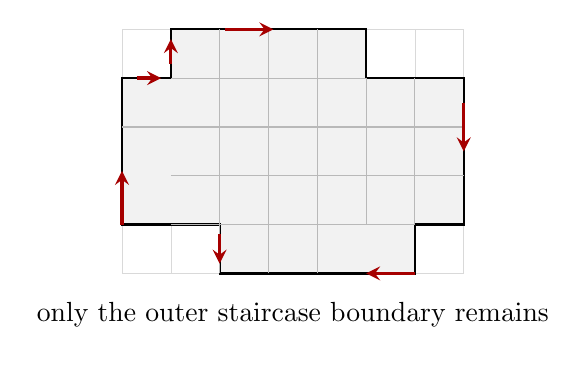
\begin{tikzpicture}[scale=0.62, >=stealth]
    \draw[step=1, gray!30, very thin] (0,0) grid (7,5);

    \draw[fill=gray!10, thick]
        (0,1) -- (0,4) -- (1,4) -- (1,5) -- (5,5) -- (5,4) --
        (7,4) -- (7,1) -- (6,1) -- (6,0) -- (2,0) -- (2,1) -- cycle;

    \draw[gray!55] (1,1) -- (6,1);
    \draw[gray!55] (1,2) -- (7,2);
    \draw[gray!55] (0,3) -- (7,3);
    \draw[gray!55] (1,4) -- (5,4);
    \draw[gray!55] (2,0) -- (2,5);
    \draw[gray!55] (3,0) -- (3,5);
    \draw[gray!55] (4,0) -- (4,5);
    \draw[gray!55] (5,1) -- (5,4);
    \draw[gray!55] (6,1) -- (6,4);

    \draw[->, very thick, red!65!black] (0,1) -- (0,2.1);
    \draw[->, very thick, red!65!black] (0.3,4) -- (0.8,4);
    \draw[->, very thick, red!65!black] (1,4.3) -- (1,4.8);
    \draw[->, very thick, red!65!black] (2.1,5) -- (3.1,5);
    \draw[->, very thick, red!65!black] (7,3.5) -- (7,2.5);
    \draw[->, very thick, red!65!black] (6,0) -- (5,0);
    \draw[->, very thick, red!65!black] (2,0.8) -- (2,0.2);

    \node at (3.5,-0.85) {only the outer staircase boundary remains};
\end{tikzpicture}
\caption{For a finite union of rectangles, all interior edges cancel in pairs.}
\end{figure}

This cancellation is the two-dimensional version of a familiar one-dimensional fact.
When we add
\[
    \int_{x_0}^{x_1}f'(x)\,dx
    +
    \int_{x_1}^{x_2}f'(x)\,dx
    +
    \cdots
    +
    \int_{x_{n-1}}^{x_n}f'(x)\,dx,
\]
the intermediate endpoint values cancel:
\[
    f(x_1)-f(x_0)+f(x_2)-f(x_1)+\cdots+f(x_n)-f(x_{n-1})
    =
    f(x_n)-f(x_0).
\]
Green's theorem does the same thing one dimension higher.  Interior edges are the new
intermediate endpoints.

\subsection{Curved boundaries by slicing}

Rectangles explain the theorem's engine.  Curved boundaries require one more idea:
slice the region into pieces where the one-variable Fundamental Theorem of Calculus
can still see the edge differences.

Let
\[
    R=\{(x,y):a\le x\le b,\ g(x)\le y\le h(x)\},
\]
where \(g\) and \(h\) are smooth.  This is a vertically simple region.

For the form
\[
    P\,dx,
\]
the vertical sides do not contribute, because \(dx=0\) there.  The bottom curve is
walked from \(a\) to \(b\), and the top curve is walked from \(b\) to \(a\).  Therefore
\[
\begin{aligned}
    \oint_{\partial R}P\,dx
    &=
    \int_a^b P(x,g(x))\,dx
    -
    \int_a^b P(x,h(x))\,dx\\
    &=
    -\int_a^b\bigl(P(x,h(x))-P(x,g(x))\bigr)\,dx.
\end{aligned}
\]
For each fixed \(x\), the Fundamental Theorem of Calculus gives
\[
    P(x,h(x))-P(x,g(x))
    =
    \int_{g(x)}^{h(x)}P_y(x,y)\,dy.
\]
So
\[
\boxed{
    \oint_{\partial R}P\,dx
    =
    -\int_a^b\int_{g(x)}^{h(x)}P_y(x,y)\,dy\,dx.
}
\]

The \(Q\,dy\) part is proved the same way on a horizontally simple region
\[
    R=\{(x,y):c\le y\le d,\ \ell(y)\le x\le r(y)\}.
\]
The horizontal sides do not contribute, because \(dy=0\).  The right boundary is
walked upward, and the left boundary is walked downward.  Thus
\[
\begin{aligned}
    \oint_{\partial R}Q\,dy
    &=
    \int_c^d Q(r(y),y)\,dy
    -
    \int_c^d Q(\ell(y),y)\,dy\\
    &=
    \int_c^d\bigl(Q(r(y),y)-Q(\ell(y),y)\bigr)\,dy\\
    &=
    \int_c^d\int_{\ell(y)}^{r(y)}Q_x(x,y)\,dx\,dy.
\end{aligned}
\]
So
\[
\boxed{
    \oint_{\partial R}Q\,dy
    =
    \iint_R Q_x\,dA.
}
\]

If a region can be cut into finitely many pieces that are both vertically and horizontally
simple, then the two formulas apply on each piece.  Adding the pieces cancels the
new internal boundaries, exactly as with rectangles.

This proves Green's theorem for many familiar regions: disks, ellipses, polygons, and
regions with piecewise smooth boundary after a finite number of cuts.

\subsection{Curved boundaries by approximation}

There is another way to picture the last step.  Overlay a fine grid on a curved region
\(R\).  Keep the grid squares that lie inside.  The result is a staircase region \(R_h\)
made from finitely many rectangles.  For \(R_h\),
\[
    \int_{\partial R_h}\omega=\int_{R_h}d\omega
\]
is already proved.

As the grid becomes finer, two things happen.

First, the area integral over \(R_h\) approaches the area integral over \(R\):
\[
    \int_{R_h}d\omega\longrightarrow \int_R d\omega.
\]
Continuity of \(Q_x-P_y\) keeps the values from jumping unpredictably in the thin
strip near the boundary.

Second, the staircase boundary approaches the curved boundary.  On a smooth arc, a
tiny stair step has almost the same first-order effect as the tiny curve segment it
replaces.  Adding those small differences along the boundary makes the boundary
integral approach
\[
    \int_{\partial R}\omega.
\]

\begin{figure}[h]
\centering
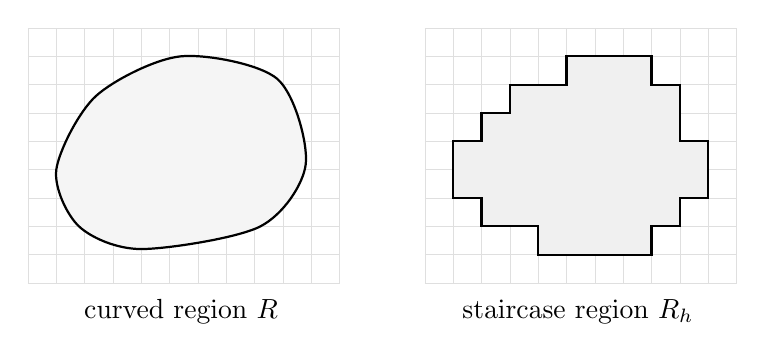
\begin{tikzpicture}[scale=0.72, >=stealth]
    \begin{scope}
        \draw[step=0.5, gray!25, very thin] (-0.5,-0.5) grid (5,4);

        \draw[fill=gray!8, thick]
            plot[smooth cycle] coordinates {
                (0.4,0.5)
                (1.5,0.1)
                (3.6,0.5)
                (4.4,1.6)
                (3.9,3.1)
                (2.2,3.5)
                (0.7,2.8)
                (0.0,1.5)
            };

        \node at (2.2,-1.0) {curved region \(R\)};
    \end{scope}

    \begin{scope}[shift={(7,0)}]
        \draw[step=0.5, gray!25, very thin] (-0.5,-0.5) grid (5,4);

        \draw[fill=gray!12, thick]
            (0.5,0.5) -- (1.5,0.5) -- (1.5,0.0) -- (3.5,0.0) --
            (3.5,0.5) -- (4.0,0.5) -- (4.0,1.0) -- (4.5,1.0) --
            (4.5,2.0) -- (4.0,2.0) -- (4.0,3.0) -- (3.5,3.0) --
            (3.5,3.5) -- (2.0,3.5) -- (2.0,3.0) -- (1.0,3.0) --
            (1.0,2.5) -- (0.5,2.5) -- (0.5,2.0) -- (0.0,2.0) --
            (0.0,1.0) -- (0.5,1.0) -- cycle;

        \node at (2.2,-1.0) {staircase region \(R_h\)};
    \end{scope}
\end{tikzpicture}
\caption{A curved region can be approximated by regions made from rectangles.}
\end{figure}

This approximation picture is not a full proof by itself.  It tells us where the
hypotheses enter.

The boundary must be piecewise smooth so the staircase boundary really approaches a
curve with well-defined line integrals.  The partial derivatives must be continuous so
the interior integral behaves predictably as the boundary strip shrinks.  The boundary
must include every component so cancellation does not leave a hidden edge behind.

Those words are carrying real work.  If we reverse orientation, hide a singularity,
forget a hole, or ask the theorem to handle a boundary too wild for our definition of
line integral, the formula can give the wrong sign, the wrong number, or no number at
all.  The proof has shown us exactly where to look for the trouble.

\section{Warning examples}
\label{sec:14.6}

The proof in Section \ref{sec:14.5} was built from rectangles, cancellation, and limiting
curved boundaries.  Each hypothesis in Green's theorem protects one of those steps.
The warnings below are not exceptions to the theorem.  They are examples where the
theorem's words have been changed.

\subsection{Reversing orientation changes the sign}

Take the unit square
\[
    R=[0,1]\times[0,1],
\]
and the form
\[
    \omega=x\,dy.
\]
Then
\[
    d\omega=dx\wedge dy,
\]
so
\[
    \int_R d\omega=\operatorname{Area}(R)=1.
\]

Now compute the boundary integral with positive orientation.  The bottom and top
edges have \(dy=0\).  The left edge has \(x=0\).  Only the right edge contributes.
There,
\[
    x=1,
    \qquad
    0\le y\le1.
\]
So
\[
    \oint_{\partial R}x\,dy
    =
    \int_0^1 1\,dy
    =
    1.
\]
This matches Green's theorem.

If we walk the same boundary clockwise, the right edge is walked downward:
\[
    1\ge y\ge0.
\]
The integral becomes
\[
    \int_1^0 1\,dy=-1.
\]
The interior integral is still
\[
    \int_R dx\wedge dy=1.
\]
So the clockwise boundary gives the wrong sign:
\[
\boxed{
    \int_{-\partial R}\omega=-\int_{\partial R}\omega.
}
\]

The theorem did not fail.  Its orientation condition was ignored.  Positive orientation
means the region stays on the left.

\subsection{A singularity inside the region cannot be hidden}

Now return to the angle form
\[
    \alpha=\frac{-y\,dx+x\,dy}{x^2+y^2}.
\]
It is defined on the punctured plane
\[
    \mathbb R^2\setminus\{(0,0)\},
\]
but not at the origin.

Where it is defined, write
\[
    P(x,y)=\frac{-y}{x^2+y^2},
    \qquad
    Q(x,y)=\frac{x}{x^2+y^2}.
\]
A direct calculation gives
\[
    Q_x=
    \frac{y^2-x^2}{(x^2+y^2)^2}
\]
and
\[
    P_y=
    \frac{y^2-x^2}{(x^2+y^2)^2}.
\]
Thus
\[
    Q_x-P_y=0
\]
away from the origin, so
\[
    d\alpha=0
\]
on the punctured plane.

Now integrate around the unit circle
\[
    C:\quad x=\cos t,\qquad y=\sin t,\qquad 0\le t\le2\pi,
\]
oriented counterclockwise.  Then
\[
    dx=-\sin t\,dt,
    \qquad
    dy=\cos t\,dt.
\]
The numerator becomes
\[
\begin{aligned}
    -y\,dx+x\,dy
    &=
    -(\sin t)(-\sin t\,dt)+(\cos t)(\cos t\,dt)\\
    &=
    \sin^2t\,dt+\cos^2t\,dt\\
    &=
    dt.
\end{aligned}
\]
The denominator is
\[
    x^2+y^2=1.
\]
Therefore
\[
\boxed{
    \oint_C\alpha
    =
    \int_0^{2\pi}dt
    =
    2\pi.
}
\]

If we tried to apply Green's theorem to the disk bounded by \(C\), we would be tempted
to write
\[
    \oint_C\alpha
    =
    \iint_{\text{disk}}0\,dA
    =
    0.
\]
But the boundary integral is \(2\pi\).

The missing hypothesis is not small.  Green's theorem requires the form to be defined
with continuous first partial derivatives on an open region containing the whole disk.
The origin is inside the disk, and \(\alpha\) is not defined there.  The circulation is
hiding at that missing point.

\begin{figure}[h]
\centering
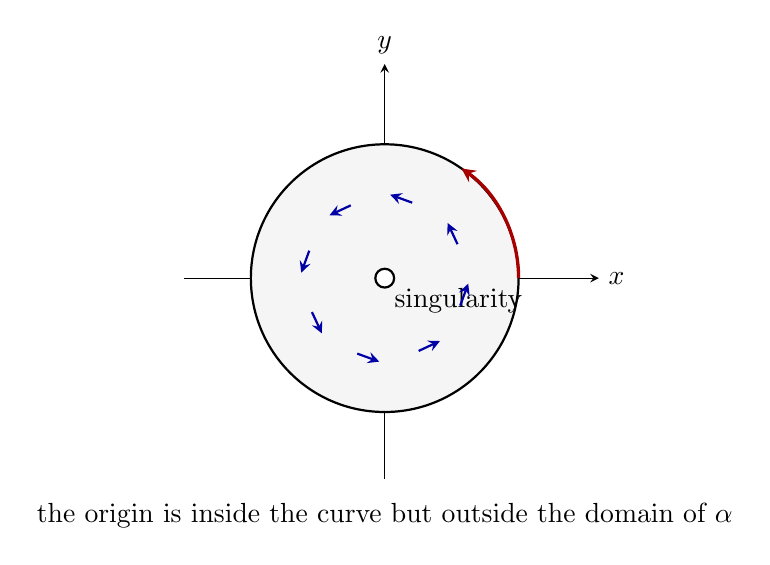
\begin{tikzpicture}[scale=0.85, >=stealth]
    \draw[->] (-3.0,0) -- (3.2,0) node[right] {\(x\)};
    \draw[->] (0,-3.0) -- (0,3.2) node[above] {\(y\)};

    \draw[thick, fill=gray!8] (0,0) circle (2);
    \draw[->, very thick, red!65!black] (2,0) arc[start angle=0,end angle=55,radius=2];

    \fill[white] (0,0) circle (4pt);
    \draw[thick] (0,0) circle (4pt);
    \node[below right] at (0,0) {singularity};

    \foreach \ang in {25,70,115,160,205,250,295,340} {
        \draw[->, blue!65!black, thick]
            ({1.2*cos(\ang)},{1.2*sin(\ang)})
            -- ++({-0.35*sin(\ang)},{0.35*cos(\ang)});
    }

    \node at (0,-3.55) {the origin is inside the curve but outside the domain of \(\alpha\)};
\end{tikzpicture}
\caption{A singularity inside the region can carry circulation even when \(d\alpha=0\)
away from it.}
\end{figure}

\subsection{A hole must be included in the boundary}

A hole is not only missing area.  It is also an extra boundary curve.

Let \(A\) be the annulus
\[
    1\le x^2+y^2\le4.
\]
Use the area form
\[
    \omega=x\,dy.
\]
Since
\[
    d\omega=dx\wedge dy,
\]
Green's theorem predicts
\[
    \oint_{\partial A}x\,dy
    =
    \operatorname{Area}(A)
    =
    4\pi-\pi
    =
    3\pi.
\]

The boundary of \(A\) has two pieces:

\[
\begin{array}{c|c|c}
\text{piece} & \text{radius} & \text{positive orientation}\\ \hline
C_{\mathrm{out}} & 2 & \text{counterclockwise}\\[1mm]
C_{\mathrm{in}} & 1 & \text{clockwise}
\end{array}
\]

For the outer circle,
\[
    x=2\cos t,
    \qquad
    y=2\sin t,
    \qquad
    0\le t\le2\pi.
\]
Then
\[
    dy=2\cos t\,dt,
\]
so
\[
\begin{aligned}
    \int_{C_{\mathrm{out}}}x\,dy
    &=
    \int_0^{2\pi}(2\cos t)(2\cos t)\,dt\\
    &=
    4\int_0^{2\pi}\cos^2t\,dt\\
    &=
    4\pi.
\end{aligned}
\]

For the inner boundary, positive orientation is clockwise.  Use
\[
    x=\cos t,
    \qquad
    y=-\sin t,
    \qquad
    0\le t\le2\pi.
\]
Then
\[
    dy=-\cos t\,dt,
\]
and
\[
\begin{aligned}
    \int_{C_{\mathrm{in}}}x\,dy
    &=
    \int_0^{2\pi}(\cos t)(-\cos t)\,dt\\
    &=
    -\pi.
\end{aligned}
\]

Therefore
\[
\boxed{
    \oint_{\partial A}x\,dy
    =
    4\pi-\pi
    =
    3\pi.
}
\]
This matches the area of the annulus.

If we used only the outer circle, we would get
\[
    4\pi,
\]
the area of the filled disk of radius \(2\), not the area of the annulus.  The inner
boundary subtracts the missing disk.

\begin{figure}[h]
\centering
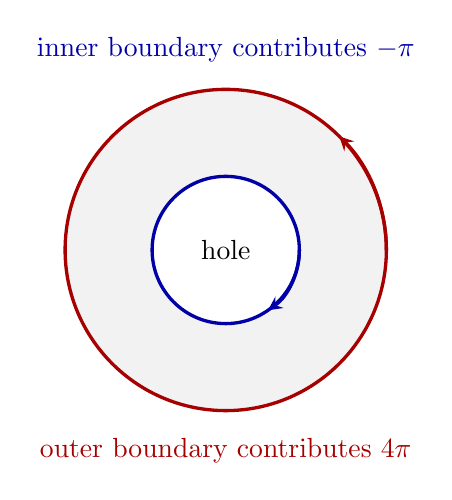
\begin{tikzpicture}[scale=0.85, >=stealth]
    \draw[fill=gray!10, even odd rule]
        (0,0) circle (2.4)
        (0,0) circle (1.1);

    \draw[very thick, red!65!black] (0,0) circle (2.4);
    \draw[->, very thick, red!65!black] (2.4,0) arc[start angle=0,end angle=45,radius=2.4];

    \draw[very thick, blue!65!black] (0,0) circle (1.1);
    \draw[->, very thick, blue!65!black] (1.1,0) arc[start angle=0,end angle=-55,radius=1.1];

    \node[red!65!black] at (0,-3.0) {outer boundary contributes \(4\pi\)};
    \node[blue!65!black] at (0,3.0) {inner boundary contributes \(-\pi\)};
    \node at (0,0) {hole};
\end{tikzpicture}
\caption{The boundary of an annulus has two components.  The inner one is oriented
clockwise.}
\end{figure}

This is the same cancellation idea from the proof.  A hole creates a boundary that does
not cancel with a neighboring piece.  It must be counted.

\subsection{A jump inside the region is a hidden edge}

Green's theorem also requires \(P\) and \(Q\) to have continuous first partial
derivatives.  A jump inside the region behaves like a boundary we forgot to draw.

Let
\[
    R=[-1,1]\times[0,1],
\]
and define
\[
    \omega=Q(x,y)\,dy,
    \qquad
    Q(x,y)=
    \begin{cases}
    0, & x\le0,\\
    1, & x>0.
    \end{cases}
\]
The form jumps across the vertical line
\[
    x=0.
\]
It is not \(C^1\).

Compute the boundary integral.  On the bottom and top edges, \(dy=0\).  On the left
edge, \(Q=0\).  On the right edge, \(Q=1\), and \(y\) goes from \(0\) to \(1\).  Thus
\[
\boxed{
    \oint_{\partial R}\omega=1.
}
\]

Away from the jump line,
\[
    Q_x=0.
\]
If we illegally pretended that
\[
    d\omega=0
\]
everywhere, then the interior integral would be
\[
    \iint_R 0\,dA=0.
\]
That is not the boundary integral.

The missing contribution lives on the internal jump line.  Smoothness prevents a
hidden edge from appearing inside the region.

\subsection{A boundary can be too rough for the theorem as stated}

The boundary condition also matters.  Green's theorem in this chapter is stated for
boundaries made from finitely many piecewise smooth simple closed curves.  That
condition guarantees that
\[
    \int_{\partial R}\omega
\]
is a finite sum of ordinary line integrals.

Consider a square pond from which infinitely many tiny circular islands have been
removed.  Let the outer square be
\[
    S=[0,1]\times[0,1],
\]
and remove disjoint disks
\[
    D_1,D_2,D_3,\ldots
\]
lying inside the square.  Suppose their areas add to a finite number:
\[
    \sum_{n=1}^{\infty}\operatorname{Area}(D_n)<1.
\]
The remaining region is
\[
    R=S\setminus\bigcup_{n=1}^{\infty}D_n.
\]

For the form
\[
    \omega=x\,dy,
\]
we have
\[
    d\omega=dx\wedge dy.
\]
For a finite number of removed disks, Green's theorem says
\[
    \oint_{\partial R_N}x\,dy
    =
    1-\sum_{n=1}^{N}\operatorname{Area}(D_n),
\]
because the outer square contributes \(1\), and each clockwise inner circle subtracts
the area of its disk.

If there are infinitely many islands, the expected answer would be
\[
    1-\sum_{n=1}^{\infty}\operatorname{Area}(D_n).
\]
But now the boundary is not a finite collection of curves.  It has infinitely many
components:
\[
    \partial S,\quad \partial D_1,\quad \partial D_2,\quad \partial D_3,\ldots
\]
The boundary integral is no longer a finite sum of line integrals.  It needs an infinite
series of boundary contributions, and convergence has to be checked.

So the elementary theorem stops before this example.  The formula may still be true
under extra assumptions, but it is no longer covered by the statement we proved.  The
word ``finitely'' is protecting us from an infinite boundary sum hidden in the notation
\[
    \int_{\partial R}.
\]

An even rougher boundary, such as a snowflake-shaped curve with infinite length and
no ordinary tangent at most points, creates a different problem: the line integral along
the boundary may not be defined by the piecewise smooth parametrizations introduced
in Chapter \ref{ch:13}.  Again, Green's theorem has not failed.  Its hypotheses have
not been met.

\subsection{What the warnings have in common}

Each warning points back to the proof.

\[
\begin{array}{c|c}
\text{What goes wrong} & \text{Where the proof breaks}\\ \hline
\text{orientation is reversed} & \text{the surviving boundary has the wrong sign}\\[1mm]
\text{a singularity lies inside} & \text{the form is not defined on the region}\\[1mm]
\text{a hole is ignored} & \text{an uncanceled boundary component is missing}\\[1mm]
\text{the coefficients jump} & \text{there is a hidden internal edge}\\[1mm]
\text{the boundary is too rough} & \text{the boundary integral is not a finite smooth sum}
\end{array}
\]

The proof was not only a justification.  It was a diagnostic tool.  It tells us what to
check before trusting the formula.

Green's theorem is a theorem about flat regions.  But its real message is larger:
boundary measurements can equal interior measurements of a derivative.  The next
time that pattern appears, the inside will not be a plane region.  It will be a surface in
space.  Then even the word ``boundary'' will need care, because a surface has two
sides, and choosing one side will decide the sign of everything that crosses it.
\section{Chapter review and applications}
\label{sec:14.7}

Green's theorem began with a small rectangle.  Opposite sides compared the field in
two directions, and the surviving coefficient was
\[
    Q_x-P_y.
\]
After adding many rectangles, every interior edge canceled.  What remained was the
boundary of the whole region.

That cancellation is the heart of the chapter:
\[
\boxed{
    \int_{\partial R}\omega=\int_R d\omega.
}
\]
The rest is learning to choose the right \(1\)-form \(\omega\), the right orientation, and
the right region.

\subsection{One theorem, several questions}

A boundary curve can answer different questions.  The same curve and the same vector
field can ask for circulation, flux, or area.  Green's theorem helps only after we know
which question we are asking.

\[
\begin{array}{c|c|c}
\text{Question} & \text{Boundary form} & \text{Interior form} \\ \hline
\text{circulation of } \mathbf F=(M,N)
&
M\,dx+N\,dy
&
(N_x-M_y)\,dx\wedge dy
\\[2mm]
\text{outward flux of } \mathbf F=(M,N)
&
M\,dy-N\,dx
&
(M_x+N_y)\,dx\wedge dy
\\[2mm]
\text{area of }R
&
x\,dy
&
dx\wedge dy
\\[2mm]
\text{area of }R
&
-y\,dx
&
dx\wedge dy
\\[2mm]
\text{area of }R
&
\dfrac12(-y\,dx+x\,dy)
&
dx\wedge dy
\end{array}
\]

The same theorem sits behind every row:
\[
    \int_{\partial R}\omega=\int_R d\omega.
\]
The form \(\omega\) decides what the boundary is measuring.

\begin{example}[The same field, two different boundary questions]
Let
\[
    R=[0,2]\times[0,1],
\]
with positive orientation, and let
\[
    \mathbf F(x,y)=(M,N)=(xy,\;x^2-y).
\]

First ask for circulation:
\[
    \oint_{\partial R}\mathbf F\cdot d\mathbf r
    =
    \oint_{\partial R}xy\,dx+(x^2-y)\,dy.
\]
Here
\[
    P=xy,
    \qquad
    Q=x^2-y.
\]
So
\[
    Q_x-P_y=2x-x=x.
\]
Green's theorem gives
\[
\begin{aligned}
    \oint_{\partial R}xy\,dx+(x^2-y)\,dy
    &=
    \iint_R x\,dA\\
    &=
    \int_0^2\int_0^1 x\,dy\,dx\\
    &=
    \int_0^2 x\,dx\\
    &=2.
\end{aligned}
\]
Thus
\[
\boxed{
    \text{circulation}=2.
}
\]

Now ask for outward flux:
\[
    \oint_{\partial R}\mathbf F\cdot\mathbf n\,ds.
\]
The flux form is
\[
    M\,dy-N\,dx
    =
    xy\,dy-(x^2-y)\,dx.
\]
Green's theorem in flux form gives
\[
    \oint_{\partial R}\mathbf F\cdot\mathbf n\,ds
    =
    \iint_R(M_x+N_y)\,dA.
\]
Since
\[
    M_x=y,
    \qquad
    N_y=-1,
\]
we get
\[
\begin{aligned}
    \oint_{\partial R}\mathbf F\cdot\mathbf n\,ds
    &=
    \iint_R(y-1)\,dA\\
    &=
    \int_0^2\int_0^1(y-1)\,dy\,dx\\
    &=
    \int_0^2\left(\frac12-1\right)dx\\
    &=-1.
\end{aligned}
\]
So
\[
\boxed{
    \text{outward flux}=-1.
}
\]

The same field and the same rectangle gave two different answers because circulation
and flux are different boundary measurements.
\end{example}

\subsection{A checklist before using Green's theorem}

Before applying
\[
    \int_{\partial R}\omega=\int_Rd\omega,
\]
pause long enough to check four things.

\[
\begin{array}{c|l}
\text{Check} & \text{What it protects} \\ \hline
\text{positive orientation} & \text{the sign of the boundary integral}\\[1mm]
\text{all boundary components} & \text{holes and inner boundaries}\\[1mm]
\omega \text{ is } C^1 \text{ near } R & \text{no hidden jumps or singularities}\\[1mm]
\partial R \text{ is piecewise smooth and finite} & \text{the boundary integral is a finite sum}
\end{array}
\]

For a region without holes, positive orientation means counterclockwise.  For a region
with holes, the outer boundary is counterclockwise and each inner boundary is
clockwise.  That one rule says the same thing everywhere:

\[
    \text{as you walk, the region stays on your left.}
\]

\subsection{Area from a boundary curve}

Green's theorem can turn a boundary walk into an area calculation.  Since
\[
    d\left(\frac12(-y\,dx+x\,dy)\right)=dx\wedge dy,
\]
a positively oriented simple closed curve \(C=\partial R\) satisfies
\[
\boxed{
    \operatorname{Area}(R)
    =
    \frac12\oint_C(-y\,dx+x\,dy).
}
\]

This formula becomes especially useful when the boundary is known but the region is
awkward.

\begin{example}[The shoelace formula from Green's theorem]
A surveyor records the vertices of a small lot, in counterclockwise order:
\[
    (0,0),\qquad
    (4,1),\qquad
    (5,4),\qquad
    (2,5),\qquad
    (-1,3).
\]
The boundary is made of straight line segments.

On one segment from
\[
    (x_i,y_i)
    \quad\text{to}\quad
    (x_{i+1},y_{i+1}),
\]
write
\[
    x(t)=x_i+t(x_{i+1}-x_i),
    \qquad
    y(t)=y_i+t(y_{i+1}-y_i),
    \qquad
    0\le t\le1.
\]
Then
\[
    dx=(x_{i+1}-x_i)\,dt,
    \qquad
    dy=(y_{i+1}-y_i)\,dt.
\]
So
\[
\begin{aligned}
\int_{\text{edge}}(-y\,dx+x\,dy)
&=
\int_0^1
\Bigl[
-(y_i+t\Delta y)\Delta x
+
(x_i+t\Delta x)\Delta y
\Bigr]dt\\
&=
x_i\Delta y-y_i\Delta x\\
&=
x_i y_{i+1}-x_{i+1}y_i.
\end{aligned}
\]
Adding all edges gives
\[
\boxed{
    \operatorname{Area}(R)
    =
    \frac12
    \left|
    \sum_{i=1}^n
    (x_i y_{i+1}-x_{i+1}y_i)
    \right|,
}
\]
where the last point is followed by the first:
\[
    (x_{n+1},y_{n+1})=(x_1,y_1).
\]
This is the shoelace formula.

For the lot above,
\[
\begin{aligned}
\sum (x_i y_{i+1}-x_{i+1}y_i)
&=
(0\cdot1-4\cdot0)\\
&\quad +(4\cdot4-5\cdot1)\\
&\quad +(5\cdot5-2\cdot4)\\
&\quad +(2\cdot3-(-1)\cdot5)\\
&\quad +((-1)\cdot0-0\cdot3)\\
&=
0+11+17+11+0\\
&=39.
\end{aligned}
\]
Therefore
\[
\boxed{
    \operatorname{Area}(R)=\frac{39}{2}.
}
\]
A formula often taught as a polygon trick is really Green's theorem in disguise.
\end{example}

\subsection{A polar area formula from the same boundary form}

The same area form also explains the familiar polar area formula.

Suppose a positively oriented boundary is written in polar form as
\[
    x=r(\theta)\cos\theta,
    \qquad
    y=r(\theta)\sin\theta,
    \qquad
    0\le \theta\le 2\pi.
\]
Then
\[
    dx=(r'\cos\theta-r\sin\theta)\,d\theta
\]
and
\[
    dy=(r'\sin\theta+r\cos\theta)\,d\theta.
\]
Compute the boundary form:
\[
\begin{aligned}
-y\,dx+x\,dy
&=
-r\sin\theta(r'\cos\theta-r\sin\theta)\,d\theta\\
&\quad
+r\cos\theta(r'\sin\theta+r\cos\theta)\,d\theta\\
&=
r^2(\sin^2\theta+\cos^2\theta)\,d\theta\\
&=
r^2\,d\theta.
\end{aligned}
\]
Thus
\[
\boxed{
    \operatorname{Area}(R)
    =
    \frac12\int_0^{2\pi}r(\theta)^2\,d\theta.
}
\]

\begin{example}[A rounded triangular lake]
A drone traces the boundary of a lake whose polar equation is
\[
    r(\theta)=3+\cos(3\theta),
    \qquad
    0\le \theta\le2\pi.
\]
Since
\[
    r(\theta)>0
\]
for all \(\theta\), the curve does not pass through the origin.  The area enclosed is
\[
\begin{aligned}
A
&=
\frac12\int_0^{2\pi}(3+\cos3\theta)^2\,d\theta\\
&=
\frac12\int_0^{2\pi}
\left(9+6\cos3\theta+\cos^2 3\theta\right)d\theta.
\end{aligned}
\]
Now
\[
    \int_0^{2\pi}\cos3\theta\,d\theta=0
\]
and
\[
    \int_0^{2\pi}\cos^2 3\theta\,d\theta=\pi.
\]
Therefore
\[
\begin{aligned}
A
&=
\frac12(18\pi+\pi)\\
&=
\frac{19\pi}{2}.
\end{aligned}
\]
So
\[
\boxed{
    A=\frac{19\pi}{2}.
}
\]

\begin{figure}[h]
\centering
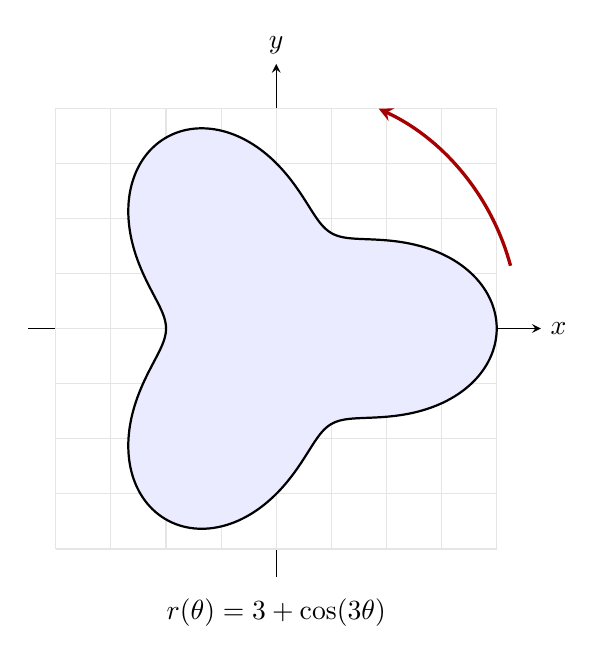
\begin{tikzpicture}[scale=0.7, >=stealth]
    \draw[->] (-4.5,0) -- (4.8,0) node[right] {\(x\)};
    \draw[->] (0,-4.5) -- (0,4.8) node[above] {\(y\)};

    \draw[gray!20, step=1] (-4,-4) grid (4,4);

    \draw[thick, fill=blue!8, domain=0:360, samples=360, smooth, variable=\t]
        plot ({(3+cos(3*\t))*cos(\t)}, {(3+cos(3*\t))*sin(\t)});

    % A clean, distinct orientation arrow hovering safely outside the boundary
    \draw[->, very thick, red!65!black]
        (15:4.4) arc[start angle=15, end angle=65, radius=4.4];

    \node at (0,-5.15) {\(r(\theta)=3+\cos(3\theta)\)};
\end{tikzpicture}
\caption{A polar boundary can give area without describing the region by inequalities.}
\end{figure}
\end{example}

\subsection{Project: area from a measured boundary curve}

A curve can be known from measurements instead of from a clean formula.  This project
uses Green's theorem to estimate area from boundary data.

Suppose a drone flies once counterclockwise around a pond and records points
\[
    (x_1,y_1),(x_2,y_2),\ldots,(x_n,y_n)
\]
at equally spaced times.  Connect consecutive points by straight segments, and connect
the last point back to the first.

\begin{enumerate}
\item Use
\[
    \operatorname{Area}
    =
    \frac12
    \left|
    \sum_{i=1}^n
    (x_i y_{i+1}-x_{i+1}y_i)
    \right|
\]
to estimate the pond's area.

\item Explain why the estimate improves as the drone records more points, assuming the
boundary is smooth.

\item Repeat the computation using
\[
    \operatorname{Area}=\oint_C x\,dy.
\]
For a straight segment from \((x_i,y_i)\) to \((x_{i+1},y_{i+1})\), show that
\[
    \int_{\text{edge}}x\,dy
    =
    \frac{x_i+x_{i+1}}{2}(y_{i+1}-y_i).
\]
Then show that the result agrees with the shoelace formula.

\item Try the method on a boundary given parametrically by
\[
    x(t)=3\cos t+\cos 2t,
    \qquad
    y(t)=2\sin t,
    \qquad
    0\le t\le2\pi.
\]
Use
\[
    \operatorname{Area}
    =
    \frac12\int_0^{2\pi}
    \bigl(x(t)y'(t)-y(t)x'(t)\bigr)\,dt.
\]
\end{enumerate}

The point is not the formula alone.  The point is that area can be recovered from a
walk around the edge.

\subsection{Practice problems}

\begin{enumerate}
\item Let \(C\) be the positively oriented boundary of the rectangle
\[
    [0,3]\times[0,2].
\]
Compute
\[
    \oint_C (x^2-y)\,dx+(xy+y^3)\,dy
\]
using Green's theorem.

\item Let \(C\) be the positively oriented unit circle.  Compute
\[
    \oint_C (e^x-y)\,dx+(x+\cos y)\,dy.
\]

\item Let \(R\) be the triangle with vertices
\[
    (0,0),\qquad (3,0),\qquad (0,2).
\]
For
\[
    \mathbf F=(x+y,\;2x-y),
\]
compute the outward flux across \(\partial R\).

\item Let \(A\) be the annulus
\[
    1\le x^2+y^2\le9.
\]
Compute
\[
    \oint_{\partial A}x\,dy.
\]
Remember the orientation of the inner boundary.

\item Let
\[
    \omega=(y^2+x)\,dx+(x^2-y)\,dy.
\]
Find \(d\omega\).  Then compute
\[
    \int_{\partial R}\omega
\]
for
\[
    R=[0,1]\times[0,2].
\]

\item Let
\[
    \alpha=\frac{-y\,dx+x\,dy}{x^2+y^2}.
\]
Explain why Green's theorem cannot be applied to \(\alpha\) on the unit disk.  Then
explain why it can be applied on the annulus
\[
    \frac14\le x^2+y^2\le1.
\]

\item A closed curve \(C\) is oriented clockwise.  If
\[
    \frac12\oint_C(-y\,dx+x\,dy)=-8,
\]
what is the area enclosed by \(C\)?

\item Find a \(1\)-form
\[
    \omega=P\,dx+Q\,dy
\]
such that
\[
    d\omega=5\,dx\wedge dy.
\]
Use it to write an area-like boundary formula for
\[
    5\operatorname{Area}(R).
\]
\end{enumerate}

\subsection{What Green's theorem cannot yet do}

Green's theorem lives in the plane.  Its region \(R\) is flat, and its boundary
\[
    \partial R
\]
is a curve.  The positive orientation rule is simple: walk so the region stays on your
left.

But many boundaries in space are not edges of flat regions.  A wire loop may bound a
soap film.  The film may bend.  The same wire may bound many different surfaces.
A dome has a top side and a bottom side.  A sphere has an outside and an inside.

On a flat region, orientation could be described by left and right.  On a surface in
space, orientation becomes a choice of normal direction.  Once that choice is made, the
boundary direction has to match it.

That is the next problem.  To carry Green's theorem into space, we need to understand
surfaces, their area, their two possible sides, and how a boundary curve knows which
side has been chosen.  The surprising part is that the same short formula will survive:
\[
    \int_{\partial(\text{something})}\omega
    =
    \int_{\text{something}}d\omega.
\]
The ``something'' will no longer be only a flat region.  It will be a surface.
